\documentclass[12pt,a4paper]{article}
\renewcommand{\baselinestretch}{1.2} 
% Add necessary packages
\usepackage{amsmath} 
\usepackage{amssymb} 
\usepackage{graphicx} 
\usepackage{hyperref} 
\usepackage{geometry} 
\usepackage{float}
\usepackage{qcircuit}
\usepackage{url}
\usepackage{braket}
\usepackage[nottoc,numbib]{tocbibind}
\geometry{margin=1in} 


% -------------------------------- start jupyter exported header ------------------------------------------
    \usepackage[breakable]{tcolorbox}
    \usepackage{parskip} % Stop auto-indenting (to mimic markdown behaviour)
    

    % Basic figure setup, for now with no caption control since it's done
    % automatically by Pandoc (which extracts ![](path) syntax from Markdown).
    %\usepackage{graphicx}
    % Maintain compatibility with old templates. Remove in nbconvert 6.0
    \let\Oldincludegraphics\includegraphics
    % Ensure that by default, figures have no caption (until we provide a
    % proper Figure object with a Caption API and a way to capture that
    % in the conversion process - todo).
    %\usepackage{caption}
    %\DeclareCaptionFormat{nocaption}{}
    %\captionsetup{format=nocaption,aboveskip=0pt,belowskip=0pt}

    %\usepackage{float}
    \floatplacement{figure}{H} % forces figures to be placed at the correct location
    \usepackage{xcolor} % Allow colors to be defined
    \usepackage{enumerate} % Needed for markdown enumerations to work
    %\usepackage{geometry} % Used to adjust the document margins
    %\usepackage{amsmath} % Equations
    %\usepackage{amssymb} % Equations
    \usepackage{textcomp} % defines textquotesingle
    % Hack from http://tex.stackexchange.com/a/47451/13684:
    \AtBeginDocument{%
        \def\PYZsq{\textquotesingle}% Upright quotes in Pygmentized code
    }
    \usepackage{upquote} % Upright quotes for verbatim code
    \usepackage{eurosym} % defines \euro

    \usepackage{iftex}
    \ifPDFTeX
        \usepackage[T1]{fontenc}
        \IfFileExists{alphabeta.sty}{
              \usepackage{alphabeta}
          }{
              \usepackage[mathletters]{ucs}
              \usepackage[utf8x]{inputenc}
          }
    \else
        \usepackage{fontspec}
        \usepackage{unicode-math}
    \fi

    \usepackage{fancyvrb} % verbatim replacement that allows latex
    \usepackage{grffile} % extends the file name processing of package graphics 
                         % to support a larger range
                         
    % Colors for the hyperref package
    \definecolor{urlcolor}{rgb}{0,.145,.698}
    \definecolor{linkcolor}{rgb}{.71,0.21,0.01}
    \definecolor{citecolor}{rgb}{.12,.54,.11}

    % ANSI colors
    \definecolor{ansi-black}{HTML}{3E424D}
    \definecolor{ansi-black-intense}{HTML}{282C36}
    \definecolor{ansi-red}{HTML}{E75C58}
    \definecolor{ansi-red-intense}{HTML}{B22B31}
    \definecolor{ansi-green}{HTML}{00A250}
    \definecolor{ansi-green-intense}{HTML}{007427}
    \definecolor{ansi-yellow}{HTML}{DDB62B}
    \definecolor{ansi-yellow-intense}{HTML}{B27D12}
    \definecolor{ansi-blue}{HTML}{208FFB}
    \definecolor{ansi-blue-intense}{HTML}{0065CA}
    \definecolor{ansi-magenta}{HTML}{D160C4}
    \definecolor{ansi-magenta-intense}{HTML}{A03196}
    \definecolor{ansi-cyan}{HTML}{60C6C8}
    \definecolor{ansi-cyan-intense}{HTML}{258F8F}
    \definecolor{ansi-white}{HTML}{C5C1B4}
    \definecolor{ansi-white-intense}{HTML}{A1A6B2}
    \definecolor{ansi-default-inverse-fg}{HTML}{FFFFFF}
    \definecolor{ansi-default-inverse-bg}{HTML}{000000}

    % common color for the border for error outputs.
    \definecolor{outerrorbackground}{HTML}{FFDFDF}

    % commands and environments needed by pandoc snippets
    % extracted from the output of `pandoc -s`
    \providecommand{\tightlist}{%
      \setlength{\itemsep}{0pt}\setlength{\parskip}{0pt}}
    \DefineVerbatimEnvironment{Highlighting}{Verbatim}{commandchars=\\\{\}}
    % Add ',fontsize=\small' for more characters per line
    \newenvironment{Shaded}{}{}
    \newcommand{\KeywordTok}[1]{\textcolor[rgb]{0.00,0.44,0.13}{\textbf{{#1}}}}
    \newcommand{\DataTypeTok}[1]{\textcolor[rgb]{0.56,0.13,0.00}{{#1}}}
    \newcommand{\DecValTok}[1]{\textcolor[rgb]{0.25,0.63,0.44}{{#1}}}
    \newcommand{\BaseNTok}[1]{\textcolor[rgb]{0.25,0.63,0.44}{{#1}}}
    \newcommand{\FloatTok}[1]{\textcolor[rgb]{0.25,0.63,0.44}{{#1}}}
    \newcommand{\CharTok}[1]{\textcolor[rgb]{0.25,0.44,0.63}{{#1}}}
    \newcommand{\StringTok}[1]{\textcolor[rgb]{0.25,0.44,0.63}{{#1}}}
    \newcommand{\CommentTok}[1]{\textcolor[rgb]{0.38,0.63,0.69}{\textit{{#1}}}}
    \newcommand{\OtherTok}[1]{\textcolor[rgb]{0.00,0.44,0.13}{{#1}}}
    \newcommand{\AlertTok}[1]{\textcolor[rgb]{1.00,0.00,0.00}{\textbf{{#1}}}}
    \newcommand{\FunctionTok}[1]{\textcolor[rgb]{0.02,0.16,0.49}{{#1}}}
    \newcommand{\RegionMarkerTok}[1]{{#1}}
    \newcommand{\ErrorTok}[1]{\textcolor[rgb]{1.00,0.00,0.00}{\textbf{{#1}}}}
    \newcommand{\NormalTok}[1]{{#1}}
    
    % Additional commands for more recent versions of Pandoc
    \newcommand{\ConstantTok}[1]{\textcolor[rgb]{0.53,0.00,0.00}{{#1}}}
    \newcommand{\SpecialCharTok}[1]{\textcolor[rgb]{0.25,0.44,0.63}{{#1}}}
    \newcommand{\VerbatimStringTok}[1]{\textcolor[rgb]{0.25,0.44,0.63}{{#1}}}
    \newcommand{\SpecialStringTok}[1]{\textcolor[rgb]{0.73,0.40,0.53}{{#1}}}
    \newcommand{\ImportTok}[1]{{#1}}
    \newcommand{\DocumentationTok}[1]{\textcolor[rgb]{0.73,0.13,0.13}{\textit{{#1}}}}
    \newcommand{\AnnotationTok}[1]{\textcolor[rgb]{0.38,0.63,0.69}{\textbf{\textit{{#1}}}}}
    \newcommand{\CommentVarTok}[1]{\textcolor[rgb]{0.38,0.63,0.69}{\textbf{\textit{{#1}}}}}
    \newcommand{\VariableTok}[1]{\textcolor[rgb]{0.10,0.09,0.49}{{#1}}}
    \newcommand{\ControlFlowTok}[1]{\textcolor[rgb]{0.00,0.44,0.13}{\textbf{{#1}}}}
    \newcommand{\OperatorTok}[1]{\textcolor[rgb]{0.40,0.40,0.40}{{#1}}}
    \newcommand{\BuiltInTok}[1]{{#1}}
    \newcommand{\ExtensionTok}[1]{{#1}}
    \newcommand{\PreprocessorTok}[1]{\textcolor[rgb]{0.74,0.48,0.00}{{#1}}}
    \newcommand{\AttributeTok}[1]{\textcolor[rgb]{0.49,0.56,0.16}{{#1}}}
    \newcommand{\InformationTok}[1]{\textcolor[rgb]{0.38,0.63,0.69}{\textbf{\textit{{#1}}}}}
    \newcommand{\WarningTok}[1]{\textcolor[rgb]{0.38,0.63,0.69}{\textbf{\textit{{#1}}}}}
    
    
    % Define a nice break command that doesn't care if a line doesn't already
    % exist.
    \def\br{\hspace*{\fill} \\* }
    % Math Jax compatibility definitions
    \def\gt{>}
    \def\lt{<}
    \let\Oldtex\TeX
    \let\Oldlatex\LaTeX
    \renewcommand{\TeX}{\textrm{\Oldtex}}
    \renewcommand{\LaTeX}{\textrm{\Oldlatex}}
    % Document parameters
    % Document title
    %\title{QPE\_popcount}
    
    
    
    
    
% Pygments definitions
\makeatletter
\def\PY@reset{\let\PY@it=\relax \let\PY@bf=\relax%
    \let\PY@ul=\relax \let\PY@tc=\relax%
    \let\PY@bc=\relax \let\PY@ff=\relax}
\def\PY@tok#1{\csname PY@tok@#1\endcsname}
\def\PY@toks#1+{\ifx\relax#1\empty\else%
    \PY@tok{#1}\expandafter\PY@toks\fi}
\def\PY@do#1{\PY@bc{\PY@tc{\PY@ul{%
    \PY@it{\PY@bf{\PY@ff{#1}}}}}}}
\def\PY#1#2{\PY@reset\PY@toks#1+\relax+\PY@do{#2}}

\@namedef{PY@tok@w}{\def\PY@tc##1{\textcolor[rgb]{0.73,0.73,0.73}{##1}}}
\@namedef{PY@tok@c}{\let\PY@it=\textit\def\PY@tc##1{\textcolor[rgb]{0.24,0.48,0.48}{##1}}}
\@namedef{PY@tok@cp}{\def\PY@tc##1{\textcolor[rgb]{0.61,0.40,0.00}{##1}}}
\@namedef{PY@tok@k}{\let\PY@bf=\textbf\def\PY@tc##1{\textcolor[rgb]{0.00,0.50,0.00}{##1}}}
\@namedef{PY@tok@kp}{\def\PY@tc##1{\textcolor[rgb]{0.00,0.50,0.00}{##1}}}
\@namedef{PY@tok@kt}{\def\PY@tc##1{\textcolor[rgb]{0.69,0.00,0.25}{##1}}}
\@namedef{PY@tok@o}{\def\PY@tc##1{\textcolor[rgb]{0.40,0.40,0.40}{##1}}}
\@namedef{PY@tok@ow}{\let\PY@bf=\textbf\def\PY@tc##1{\textcolor[rgb]{0.67,0.13,1.00}{##1}}}
\@namedef{PY@tok@nb}{\def\PY@tc##1{\textcolor[rgb]{0.00,0.50,0.00}{##1}}}
\@namedef{PY@tok@nf}{\def\PY@tc##1{\textcolor[rgb]{0.00,0.00,1.00}{##1}}}
\@namedef{PY@tok@nc}{\let\PY@bf=\textbf\def\PY@tc##1{\textcolor[rgb]{0.00,0.00,1.00}{##1}}}
\@namedef{PY@tok@nn}{\let\PY@bf=\textbf\def\PY@tc##1{\textcolor[rgb]{0.00,0.00,1.00}{##1}}}
\@namedef{PY@tok@ne}{\let\PY@bf=\textbf\def\PY@tc##1{\textcolor[rgb]{0.80,0.25,0.22}{##1}}}
\@namedef{PY@tok@nv}{\def\PY@tc##1{\textcolor[rgb]{0.10,0.09,0.49}{##1}}}
\@namedef{PY@tok@no}{\def\PY@tc##1{\textcolor[rgb]{0.53,0.00,0.00}{##1}}}
\@namedef{PY@tok@nl}{\def\PY@tc##1{\textcolor[rgb]{0.46,0.46,0.00}{##1}}}
\@namedef{PY@tok@ni}{\let\PY@bf=\textbf\def\PY@tc##1{\textcolor[rgb]{0.44,0.44,0.44}{##1}}}
\@namedef{PY@tok@na}{\def\PY@tc##1{\textcolor[rgb]{0.41,0.47,0.13}{##1}}}
\@namedef{PY@tok@nt}{\let\PY@bf=\textbf\def\PY@tc##1{\textcolor[rgb]{0.00,0.50,0.00}{##1}}}
\@namedef{PY@tok@nd}{\def\PY@tc##1{\textcolor[rgb]{0.67,0.13,1.00}{##1}}}
\@namedef{PY@tok@s}{\def\PY@tc##1{\textcolor[rgb]{0.73,0.13,0.13}{##1}}}
\@namedef{PY@tok@sd}{\let\PY@it=\textit\def\PY@tc##1{\textcolor[rgb]{0.73,0.13,0.13}{##1}}}
\@namedef{PY@tok@si}{\let\PY@bf=\textbf\def\PY@tc##1{\textcolor[rgb]{0.64,0.35,0.47}{##1}}}
\@namedef{PY@tok@se}{\let\PY@bf=\textbf\def\PY@tc##1{\textcolor[rgb]{0.67,0.36,0.12}{##1}}}
\@namedef{PY@tok@sr}{\def\PY@tc##1{\textcolor[rgb]{0.64,0.35,0.47}{##1}}}
\@namedef{PY@tok@ss}{\def\PY@tc##1{\textcolor[rgb]{0.10,0.09,0.49}{##1}}}
\@namedef{PY@tok@sx}{\def\PY@tc##1{\textcolor[rgb]{0.00,0.50,0.00}{##1}}}
\@namedef{PY@tok@m}{\def\PY@tc##1{\textcolor[rgb]{0.40,0.40,0.40}{##1}}}
\@namedef{PY@tok@gh}{\let\PY@bf=\textbf\def\PY@tc##1{\textcolor[rgb]{0.00,0.00,0.50}{##1}}}
\@namedef{PY@tok@gu}{\let\PY@bf=\textbf\def\PY@tc##1{\textcolor[rgb]{0.50,0.00,0.50}{##1}}}
\@namedef{PY@tok@gd}{\def\PY@tc##1{\textcolor[rgb]{0.63,0.00,0.00}{##1}}}
\@namedef{PY@tok@gi}{\def\PY@tc##1{\textcolor[rgb]{0.00,0.52,0.00}{##1}}}
\@namedef{PY@tok@gr}{\def\PY@tc##1{\textcolor[rgb]{0.89,0.00,0.00}{##1}}}
\@namedef{PY@tok@ge}{\let\PY@it=\textit}
\@namedef{PY@tok@gs}{\let\PY@bf=\textbf}
\@namedef{PY@tok@gp}{\let\PY@bf=\textbf\def\PY@tc##1{\textcolor[rgb]{0.00,0.00,0.50}{##1}}}
\@namedef{PY@tok@go}{\def\PY@tc##1{\textcolor[rgb]{0.44,0.44,0.44}{##1}}}
\@namedef{PY@tok@gt}{\def\PY@tc##1{\textcolor[rgb]{0.00,0.27,0.87}{##1}}}
\@namedef{PY@tok@err}{\def\PY@bc##1{{\setlength{\fboxsep}{\string -\fboxrule}\fcolorbox[rgb]{1.00,0.00,0.00}{1,1,1}{\strut ##1}}}}
\@namedef{PY@tok@kc}{\let\PY@bf=\textbf\def\PY@tc##1{\textcolor[rgb]{0.00,0.50,0.00}{##1}}}
\@namedef{PY@tok@kd}{\let\PY@bf=\textbf\def\PY@tc##1{\textcolor[rgb]{0.00,0.50,0.00}{##1}}}
\@namedef{PY@tok@kn}{\let\PY@bf=\textbf\def\PY@tc##1{\textcolor[rgb]{0.00,0.50,0.00}{##1}}}
\@namedef{PY@tok@kr}{\let\PY@bf=\textbf\def\PY@tc##1{\textcolor[rgb]{0.00,0.50,0.00}{##1}}}
\@namedef{PY@tok@bp}{\def\PY@tc##1{\textcolor[rgb]{0.00,0.50,0.00}{##1}}}
\@namedef{PY@tok@fm}{\def\PY@tc##1{\textcolor[rgb]{0.00,0.00,1.00}{##1}}}
\@namedef{PY@tok@vc}{\def\PY@tc##1{\textcolor[rgb]{0.10,0.09,0.49}{##1}}}
\@namedef{PY@tok@vg}{\def\PY@tc##1{\textcolor[rgb]{0.10,0.09,0.49}{##1}}}
\@namedef{PY@tok@vi}{\def\PY@tc##1{\textcolor[rgb]{0.10,0.09,0.49}{##1}}}
\@namedef{PY@tok@vm}{\def\PY@tc##1{\textcolor[rgb]{0.10,0.09,0.49}{##1}}}
\@namedef{PY@tok@sa}{\def\PY@tc##1{\textcolor[rgb]{0.73,0.13,0.13}{##1}}}
\@namedef{PY@tok@sb}{\def\PY@tc##1{\textcolor[rgb]{0.73,0.13,0.13}{##1}}}
\@namedef{PY@tok@sc}{\def\PY@tc##1{\textcolor[rgb]{0.73,0.13,0.13}{##1}}}
\@namedef{PY@tok@dl}{\def\PY@tc##1{\textcolor[rgb]{0.73,0.13,0.13}{##1}}}
\@namedef{PY@tok@s2}{\def\PY@tc##1{\textcolor[rgb]{0.73,0.13,0.13}{##1}}}
\@namedef{PY@tok@sh}{\def\PY@tc##1{\textcolor[rgb]{0.73,0.13,0.13}{##1}}}
\@namedef{PY@tok@s1}{\def\PY@tc##1{\textcolor[rgb]{0.73,0.13,0.13}{##1}}}
\@namedef{PY@tok@mb}{\def\PY@tc##1{\textcolor[rgb]{0.40,0.40,0.40}{##1}}}
\@namedef{PY@tok@mf}{\def\PY@tc##1{\textcolor[rgb]{0.40,0.40,0.40}{##1}}}
\@namedef{PY@tok@mh}{\def\PY@tc##1{\textcolor[rgb]{0.40,0.40,0.40}{##1}}}
\@namedef{PY@tok@mi}{\def\PY@tc##1{\textcolor[rgb]{0.40,0.40,0.40}{##1}}}
\@namedef{PY@tok@il}{\def\PY@tc##1{\textcolor[rgb]{0.40,0.40,0.40}{##1}}}
\@namedef{PY@tok@mo}{\def\PY@tc##1{\textcolor[rgb]{0.40,0.40,0.40}{##1}}}
\@namedef{PY@tok@ch}{\let\PY@it=\textit\def\PY@tc##1{\textcolor[rgb]{0.24,0.48,0.48}{##1}}}
\@namedef{PY@tok@cm}{\let\PY@it=\textit\def\PY@tc##1{\textcolor[rgb]{0.24,0.48,0.48}{##1}}}
\@namedef{PY@tok@cpf}{\let\PY@it=\textit\def\PY@tc##1{\textcolor[rgb]{0.24,0.48,0.48}{##1}}}
\@namedef{PY@tok@c1}{\let\PY@it=\textit\def\PY@tc##1{\textcolor[rgb]{0.24,0.48,0.48}{##1}}}
\@namedef{PY@tok@cs}{\let\PY@it=\textit\def\PY@tc##1{\textcolor[rgb]{0.24,0.48,0.48}{##1}}}

\def\PYZbs{\char`\\}
\def\PYZus{\char`\_}
\def\PYZob{\char`\{}
\def\PYZcb{\char`\}}
\def\PYZca{\char`\^}
\def\PYZam{\char`\&}
\def\PYZlt{\char`\<}
\def\PYZgt{\char`\>}
\def\PYZsh{\char`\#}
\def\PYZpc{\char`\%}
\def\PYZdl{\char`\$}
\def\PYZhy{\char`\-}
\def\PYZsq{\char`\'}
\def\PYZdq{\char`\"}
\def\PYZti{\char`\~}
% for compatibility with earlier versions
\def\PYZat{@}
\def\PYZlb{[}
\def\PYZrb{]}
\makeatother


% For linebreaks inside Verbatim environment from package fancyvrb. 
\makeatletter
    \newbox\Wrappedcontinuationbox 
    \newbox\Wrappedvisiblespacebox 
    \newcommand*\Wrappedvisiblespace {\textcolor{red}{\textvisiblespace}} 
    \newcommand*\Wrappedcontinuationsymbol {\textcolor{red}{\llap{\tiny$\m@th\hookrightarrow$}}} 
    \newcommand*\Wrappedcontinuationindent {3ex } 
    \newcommand*\Wrappedafterbreak {\kern\Wrappedcontinuationindent\copy\Wrappedcontinuationbox} 
    % Take advantage of the already applied Pygments mark-up to insert 
    % potential linebreaks for TeX processing. 
    %        {, <, #, %, $, ' and ": go to next line. 
    %        _, }, ^, &, >, - and ~: stay at end of broken line. 
    % Use of \textquotesingle for straight quote. 
    \newcommand*\Wrappedbreaksatspecials {% 
        \def\PYGZus{\discretionary{\char`\_}{\Wrappedafterbreak}{\char`\_}}% 
        \def\PYGZob{\discretionary{}{\Wrappedafterbreak\char`\{}{\char`\{}}% 
        \def\PYGZcb{\discretionary{\char`\}}{\Wrappedafterbreak}{\char`\}}}% 
        \def\PYGZca{\discretionary{\char`\^}{\Wrappedafterbreak}{\char`\^}}% 
        \def\PYGZam{\discretionary{\char`\&}{\Wrappedafterbreak}{\char`\&}}% 
        \def\PYGZlt{\discretionary{}{\Wrappedafterbreak\char`\<}{\char`\<}}% 
        \def\PYGZgt{\discretionary{\char`\>}{\Wrappedafterbreak}{\char`\>}}% 
        \def\PYGZsh{\discretionary{}{\Wrappedafterbreak\char`\#}{\char`\#}}% 
        \def\PYGZpc{\discretionary{}{\Wrappedafterbreak\char`\%}{\char`\%}}% 
        \def\PYGZdl{\discretionary{}{\Wrappedafterbreak\char`\$}{\char`\$}}% 
        \def\PYGZhy{\discretionary{\char`\-}{\Wrappedafterbreak}{\char`\-}}% 
        \def\PYGZsq{\discretionary{}{\Wrappedafterbreak\textquotesingle}{\textquotesingle}}% 
        \def\PYGZdq{\discretionary{}{\Wrappedafterbreak\char`\"}{\char`\"}}% 
        \def\PYGZti{\discretionary{\char`\~}{\Wrappedafterbreak}{\char`\~}}% 
    } 
    % Some characters . , ; ? ! / are not pygmentized. 
    % This macro makes them "active" and they will insert potential linebreaks 
    \newcommand*\Wrappedbreaksatpunct {% 
        \lccode`\~`\.\lowercase{\def~}{\discretionary{\hbox{\char`\.}}{\Wrappedafterbreak}{\hbox{\char`\.}}}% 
        \lccode`\~`\,\lowercase{\def~}{\discretionary{\hbox{\char`\,}}{\Wrappedafterbreak}{\hbox{\char`\,}}}% 
        \lccode`\~`\;\lowercase{\def~}{\discretionary{\hbox{\char`\;}}{\Wrappedafterbreak}{\hbox{\char`\;}}}% 
        \lccode`\~`\:\lowercase{\def~}{\discretionary{\hbox{\char`\:}}{\Wrappedafterbreak}{\hbox{\char`\:}}}% 
        \lccode`\~`\?\lowercase{\def~}{\discretionary{\hbox{\char`\?}}{\Wrappedafterbreak}{\hbox{\char`\?}}}% 
        \lccode`\~`\!\lowercase{\def~}{\discretionary{\hbox{\char`\!}}{\Wrappedafterbreak}{\hbox{\char`\!}}}% 
        \lccode`\~`\/\lowercase{\def~}{\discretionary{\hbox{\char`\/}}{\Wrappedafterbreak}{\hbox{\char`\/}}}% 
        \catcode`\.\active
        \catcode`\,\active 
        \catcode`\;\active
        \catcode`\:\active
        \catcode`\?\active
        \catcode`\!\active
        \catcode`\/\active 
        \lccode`\~`\~ 	
    }
\makeatother

\let\OriginalVerbatim=\Verbatim
\makeatletter
\renewcommand{\Verbatim}[1][1]{%
    %\parskip\z@skip
    \sbox\Wrappedcontinuationbox {\Wrappedcontinuationsymbol}%
    \sbox\Wrappedvisiblespacebox {\FV@SetupFont\Wrappedvisiblespace}%
    \def\FancyVerbFormatLine ##1{\hsize\linewidth
        \vtop{\raggedright\hyphenpenalty\z@\exhyphenpenalty\z@
            \doublehyphendemerits\z@\finalhyphendemerits\z@
            \strut ##1\strut}%
    }%
    % If the linebreak is at a space, the latter will be displayed as visible
    % space at end of first line, and a continuation symbol starts next line.
    % Stretch/shrink are however usually zero for typewriter font.
    \def\FV@Space {%
        \nobreak\hskip\z@ plus\fontdimen3\font minus\fontdimen4\font
        \discretionary{\copy\Wrappedvisiblespacebox}{\Wrappedafterbreak}
        {\kern\fontdimen2\font}%
    }%
    
    % Allow breaks at special characters using \PYG... macros.
    \Wrappedbreaksatspecials
    % Breaks at punctuation characters . , ; ? ! and / need catcode=\active 	
    \OriginalVerbatim[#1,codes*=\Wrappedbreaksatpunct]%
}
\makeatother

% Exact colors from NB
\definecolor{incolor}{HTML}{303F9F}
\definecolor{outcolor}{HTML}{D84315}
\definecolor{cellborder}{HTML}{CFCFCF}
\definecolor{cellbackground}{HTML}{F7F7F7}

% prompt
\makeatletter
\newcommand{\boxspacing}{\kern\kvtcb@left@rule\kern\kvtcb@boxsep}
\makeatother
\newcommand{\prompt}[4]{
    {\ttfamily\llap{{\color{#2}[#3]:\hspace{3pt}#4}}\vspace{-\baselineskip}}
}



% Prevent overflowing lines due to hard-to-break entities
\sloppy 
% Setup hyperref package
\hypersetup{
  breaklinks=true,  % so long urls are correctly broken across lines
  colorlinks=true,
  urlcolor=urlcolor,
  linkcolor=linkcolor,
  citecolor=citecolor,
  }
% Slightly bigger margins than the latex defaults

\geometry{verbose,tmargin=1in,bmargin=1in,lmargin=1in,rmargin=1in}
% -------------------------------- End jupyter export header ----------------------------------------------

\setlength{\arrayrulewidth}{0.2mm}
\setlength{\tabcolsep}{10pt}
\renewcommand{\arraystretch}{1.5}

\title{%
    Calculating the population count of a binary string on a Quantum Computer \\
    \large Exam ACIT4321 Quantum Information Technology\\
    }

\author{Bernt Moritz Schmid Olsen (s341528), Rolf Alexander Klæboe (rokla9659)}
\date{November 2024, OsloMet}


\begin{document}

\maketitle
\begin{abstract}
    In this work we explore different ways to solve the popcount problem on a Quantum Computer. The popcount problem, is an important problem in Computer Science and finding efficient ways to solve this problem on a Quantum Computer is valuable. We focus specifically on constructing circuits that find the \(j\)-th bit of the output in binary form. This means we only use n+1 qubits where n is the number of input bits. Through our work, we were able to find a general approach to solve the problem for any problem size for \(j \in \{1, 2, 3\}\) values. This involves using controlled not gates with \(2^{j-1}\) control bits. For the problem instance where \(j=2\) we were also able to find a more efficient circuit by utilizing the Quantum Fourier Transform (QFT).
\end{abstract}
\newpage
{
    \hypersetup{linkcolor=black}
    \tableofcontents
}

\section{Introduction}
The popcount problem is the problem of counting the number of set bits in a binary string. It is short for population count problem and can also be described as the bit-counting problem \cite{El_Qawasmeh} or in more general terms: finding the hamming weight of a bit string. The hamming weight is the function that counts the number of non-zero elements among a string of elements from an alphabet that has a well defined zero-symbol. \cite{HAMMING2012345}. Hamming weight is significant in quantum computing for a number of different applications such as quantum cryptography, quantum algorithms such as Grover's Search algorithm\cite{10.1145/237814.237866}, and finding energy states in Ising representations.

\subsection{Problem definition}
In this work, we worked with a specific popcount problem with some constraints. For a given string \(z = z_0 z_1 z_2 ... z_n\) of n bits, the popcount problem is to find the number of set bits in the string. The output is a positive integer that can be expressed in binary. The popcount function of a bit string \(z\) is the same as hamming weight function on \(z\), which is sometimes denoted \(\omega(z)\). 
\[
\omega(z) = z_0 + z_1 + ... + z_n = y, y = y_0y_1y_2y_3 ... y_m
\]

The function produces a bit string as output with length \(m = \lfloor log_2(n) \rfloor + 1\). We try to implement the hamming weight function for a bit string of size n for one of the output bits \(y_j\) where \(0 \le y_j \le m \). For that we can only use \(n+1\) qubits (qubit constraint) and the gates allowed to be used is the CNOT gate and any single qubit gate (gate type constraint). 

In the subsequent sections we walk trough circuits that solve specific popcount problem instances. First we work with the \(j=1\) with \(n=3\) and \(n=4\). Next, we present solutions for the \(j=2\) cases for \(n_=3\) and \(n=4\). Finally we also explain how the \(j=3\) can be solved for \(n=4\). We also explain how the solutions can generalize to any n for the specific j. 


\section{Solutions}
\subsection{Solutions for \(j=1\) popcount problems}
For an input of \(n=3\) qubits, the largest popcount is 3 corresponding to $\ket{111}$. The number of output bits is given by \(m = \lfloor log_2(3)\rfloor + 1 = 1 + 1 = 2\). The number of different input bit strings is \(2^3\). With this information we can create the truth table for the problem instance (see Table \ref{tab:ttn3j2}). From the truth table it becomes clear that to find the popcount for \(j = 1\), which is the least significant bit we need a circuit that produces \(y_1 = 1\) when \(\omega(z)\) is even and \(y_1 = 0\) when \(\omega(z)\) is odd. This is trivial to do with $n$ number of CNOT gates where each input is assigned as one of the control qubits of the \(n\) qubits and the target is set to the output bit (see Figure \ref{fig:n3j1}). In this setup the X gate is applied as many times as there are set bits in the output. Thus, if \(\omega(z)\) is odd we get \(X^{2n+1} = (X^{2})^{n} \cdot X = X\) and for when \(\omega(z)\) is even, we get Identity: \(X^{2n} = (X^2)^{n} = I^n = I\). 

The exact same approach can be used to find the solution to the \(n = 4\) problem instance. note however that this time 3 bits are needed to represent y entirely: \(m = \lfloor log_2(4)\rfloor + 1 = 2 + 1 = 3\). The truth table is found in Table \ref{tab:ttn4j2}. Note that also in this case \(\ket{y_1} = \ket{1}\) if \(\omega(z)\) is odd and \(\ket{y_1} = \ket{0}\) when \(\omega(z)\). We can thus extend the same concept with CNOT gates to this problem instance (see Figure \ref{fig:n4j1})

From the two solutions derived above, the questions of generalizing this solution to \(n \ge 1\) naturally arises. We can observe that for any \(\omega(z)\) function value (\(V_{\omega} \in \mathbb{N}\)), the least significant bit in the binary representation is always 1 if the total entire binary number is odd and 0 if it is even. This arises from the binary representation of an integer where the least significant bit is contributing the term \(2^0 = 1\) if it is set. All other terms are a multiple of 2:
\[
(z_{n-1}...z_2z_11)_2 = z_{n-1}\cdot2^{n-1} + ... + z_1\cdot2^{1} + 1 = 2(z_n\cdot2^{n-2} + ... + z_1\cdot 2^{0}) + 1 = 2N + 1
\] 
\[
(z_{n-1}...z_2z_10)_2 = z_{n-1}\cdot2^{n-1} + ... + z_1\cdot2^{1} + 0 = 2(z_n\cdot2^{n-2} + ... + z_1\cdot 2^{0}) = 2N
\] where \(N\) is some positive integer.

It is therefore clear that the solution for \(n=4\) and \(n=3\) can be extended to used for all \(n \ge 1\) with \(j=1\).


\begin{figure}[t] 
    \begin{minipage}{.45\textwidth}
        \centering 
        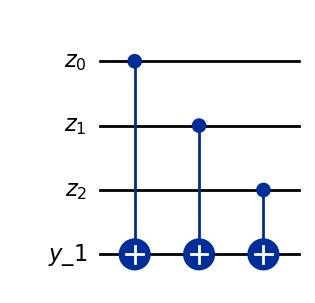
\includegraphics[width=0.8\textwidth]{Figures/j1n3.png}
        \caption{Circuit diagram for n=3, j=1 solution} 
        \label{fig:n3j1} 
    \end{minipage}
    \qquad
    \begin{minipage}{.45\textwidth}
    \centering 
        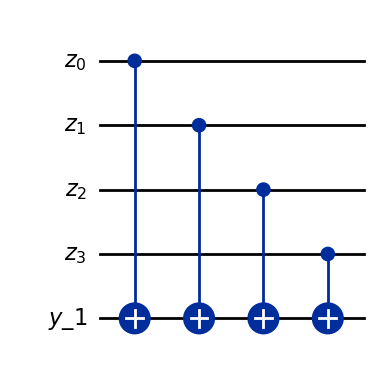
\includegraphics[width=0.8\textwidth]{Figures/n4j1_circuit_diagram.png}
        \caption{Circuit diagram for n=4, j=1 solution} 
        \label{fig:n4j1} 
    \end{minipage}  
\end{figure}


\begin{table}[t]
    \centering
    \begin{tabular}{c|c|c|c}
        $\ket{z_1,z_2,z_3}$ & $\omega(\ket{z}) = \ket{y}$ & $\ket{y_2}$ & $\ket{y_1}$\\
        $\ket{000}$& $\ket{00}$ & $\ket{0}$ & $\ket{0}$\\
        $\ket{001}$& $\ket{01}$ & $\ket{0}$ & $\ket{1}$\\
        $\ket{010}$& $\ket{01}$ & $\ket{0}$ & $\ket{1}$\\
        $\ket{011}$& $\ket{10}$ & $\ket{1}$ & $\ket{0}$\\
        $\ket{100}$& $\ket{01}$ & $\ket{0}$ & $\ket{1}$\\
        $\ket{101}$& $\ket{10}$ & $\ket{1}$ & $\ket{0}$\\
        $\ket{110}$& $\ket{10}$ & $\ket{1}$ & $\ket{0}$\\
        $\ket{111}$& $\ket{11}$ & $\ket{1}$ & $\ket{1}$\\
        
    \end{tabular}
    \caption{Truth table for \(n=3\), \(j=2, j=1\)}
    \label{tab:ttn3j2}
\end{table}

\begin{table}[t]
    \centering
    \begin{tabular}{c|c|c|c|c}
        $\ket{z_1,z_2,z_3,z_4}$ & $\omega(\ket{z}) = \ket{y}$ & $\ket{y_3}$ & $\ket{y_2}$ & $\ket{y_1}$\\
        $\ket{0000}$& $\ket{000}$ & $\ket{0}$ & $\ket{0}$ & $\ket{0}$\\
        $\ket{0001}$& $\ket{001}$ & $\ket{0}$ & $\ket{0}$ & $\ket{1}$\\
        $\ket{0010}$& $\ket{001}$ & $\ket{0}$ & $\ket{0}$ & $\ket{1}$\\
        $\ket{0011}$& $\ket{010}$ & $\ket{0}$ & $\ket{1}$ & $\ket{0}$\\
        $\ket{0100}$& $\ket{001}$ & $\ket{0}$ & $\ket{0}$ & $\ket{1}$\\
        $\ket{0101}$& $\ket{010}$ & $\ket{0}$ & $\ket{1}$ & $\ket{0}$\\
        $\ket{0110}$& $\ket{010}$ & $\ket{0}$ & $\ket{1}$ & $\ket{0}$\\
        $\ket{0111}$& $\ket{011}$ & $\ket{0}$ & $\ket{1}$ & $\ket{1}$\\
        $\ket{1000}$& $\ket{001}$ & $\ket{0}$ & $\ket{0}$ & $\ket{0}$\\
        $\ket{1001}$& $\ket{010}$ & $\ket{0}$ & $\ket{1}$ & $\ket{1}$\\
        $\ket{1010}$& $\ket{010}$ & $\ket{0}$ & $\ket{1}$ & $\ket{1}$\\
        $\ket{1011}$& $\ket{011}$ & $\ket{0}$ & $\ket{1}$ & $\ket{0}$\\
        $\ket{1100}$& $\ket{010}$ & $\ket{0}$ & $\ket{1}$ & $\ket{1}$\\
        $\ket{1101}$& $\ket{011}$ & $\ket{0}$ & $\ket{1}$ & $\ket{0}$\\
        $\ket{1110}$& $\ket{011}$ & $\ket{0}$ & $\ket{1}$ & $\ket{0}$\\
        $\ket{1111}$& $\ket{100}$ & $\ket{1}$ & $\ket{0}$ & $\ket{1}$\\
        
    \end{tabular}
    \caption{Truth table for \(n=4\), \(j=3, j=2, j=1\)}
    \label{tab:ttn4j2}
\end{table}


\subsection{Solutions to the \(j=2\) popcount problems}

In our work with this project, we found two different approaches for solving the popcount problem for \(j=2\) for any \(n \ge 2\). First we present an approach which involves using the Toffoli gate to test every possible pair of input combinations and apply the X gate as many times as there are active pairs of inputs. The other approach uses the Quantum Fourier Transform (QFT) to solve the problem. 

\subsubsection{Solving the n=3 and n=4 problems using Toffoli gates}
\label{sec:ET solutions to j=2}
In order to find the popcount for \(j = 2\), we simply count if two or more bits are $\ket{1}$. For an input of 3 qubits, we have 4 such cases as seen in Table \ref{tab:ttn3j2}. From the table we see that we want to apply \(X\) on the \(y_{j=2}\) qubit when two or more bits are $\ket{1}$, this can be achieved with three Toffoli gates arranged as given by Figure \ref{fig:n3j2}.


\begin{figure}[t] 
    \begin{minipage}{.45\textwidth}
        \centering 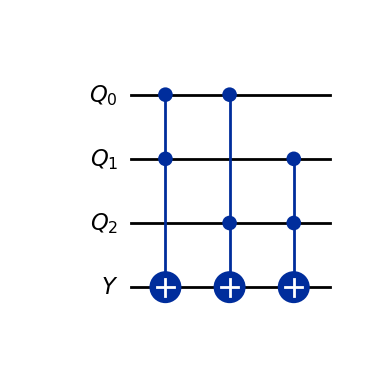
\includegraphics[width=0.8\textwidth]{Figures/n3j2_circuit_diagram.png} 
        \caption{Circuit diagram for the \(n=3\), \(j=2\) popcount problem} 
        \label{fig:n3j2}
    \end{minipage}
    \qquad
    \begin{minipage}{.45\textwidth}
        \centering 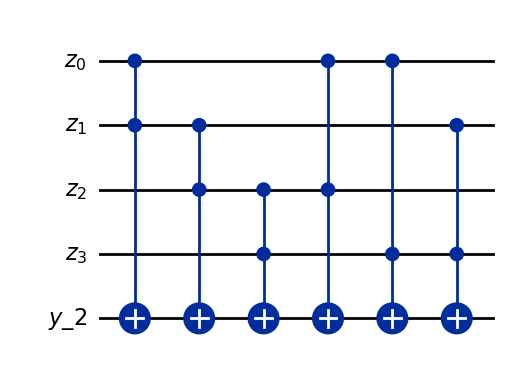
\includegraphics[width=0.8\textwidth]{Figures/toffoli_j=2_n=4.png} 
        \caption{Circuit diagram for the \(n=4\), \(j=2\) popcount problem} 
        \label{fig:n4j2_toffoli} 
    \end{minipage}
\end{figure}



%\begin{table}[h!]
%    \centering
%    \begin{tabular}{c|c}
%        $\ket{x_1,x_2,x_3}$ & $\ket{y_j}$\\
%        $\ket{000}$&  $\ket{0}$\\
%        $\ket{001}$&  $\ket{0}$\\
%        $\ket{010}$&  $\ket{0}$\\
%        $\ket{011}$&  $\ket{1}$\\
%        $\ket{100}$&  $\ket{0}$\\
%        $\ket{101}$&  $\ket{1}$\\
%        $\ket{110}$&  $\ket{1}$ \\
%        $\ket{111}$&  $\ket{1}$\\
        
%    \end{tabular}
%    \caption{Truth table for \(n=3\), \(j=2\)}
%    \label{tab:ttn3j2}
%\end{table}

The same concept applies to the case where \(n=4\). However, this time it is not enough to just check if there are at least two set bits because for the case \(\omega(1111_2) = 4 = 100_2\) the output should be 0. We should therefore analyse how the similar circuit for \(n=4\), where all possible combinations of input pairs are connected to a unique Toffoli (see Figure \ref{fig:n4j2_toffoli}), handles the different input. Henceforth, we call this approach the Exhaustive Toffoli (ET) approach. 

There are four possible hamming weights that the algorithm needs to handle: \(\omega(z) \in {0, 1, 2, 3, 4}\). When \(z = 0000_2\), the expected output is 0 and the proposed circuit (see Figure \ref{fig:n4j2_toffoli}) produces no effect on the output. The same applies for any cases where \(\omega(z) = 1\) (\(1000_2, 0100_2, 0010_2, 0001_2\)): no Toffoli gate will apply the X gate in the target if not both bits are set. For the case where two qubits are in the \(\ket{1}\) state, we can clearly deduce that only one Toffoli will be active. This is because each Toffoli is controlled by a unique pair of input bits. If there are three set bits, it is less clear because there must be more than one activated Toffoli gate. Since \(3_{10} = 11_2\), we know that \(y_2 = 1\) for \(\omega(z) = 3\). If we now look at the ways those three inputs can be combined to input a unique Toffoli, we see that it is a combination problem without repetition. The number of unique combinations of two input qubits and thus Toffoli activations, are given by the binomial coefficient:

\[
\binom{3}{2} = \frac{3\cdot2\cdot1}{2\cdot1(3-2)!} = 3
\]

This means the X gate is applied 3 times on the target qubit for any z such that \(\omega(z) = 3\): 
\[
\ket{z_n^{\omega(z)=3}} \otimes \ket{0} \; \underrightarrow{ET_4} \; \ket{z_n^{\omega(z )=3}} \otimes X^{3}\ket{0} = \ket{z_n^{\omega(z)=3}} \otimes X^2\cdot X \ket{0} = \ket{z_n^{\omega(z)=3}} \otimes \ket{1}
\]

Where \(z_n^{\omega(z)=3}\) is one of the input bit strings with three set bits and \(ET_4\) denotes the Exhaustive Toffoli circuit for four input qubits. 

The last case is when all four bits are set. But in that case all Toffoli gates must be activated. The total number of X gates applied is in this case \(\binom{4}{2} = 3\cdot2 = 6\). This is an even number, which means the effect of the X gates is canceled out because \(X^6 = (X^2)^3 = I^3 = I\). This shows that the Exhaustive Toffoli approach solves the problem. However, the original task was to solve the popcount problem with only single qubit gates or CNOT gates. For this solution to be feasible, it needs to be shown that the Toffoli gate can be decomposed with CNOT and single qubit gates. In the next section we will show how this solution fulfills the gate type constraint.

\subsubsection{Decomposition of the Toffoli gate}

Toffoli gates can be decomposed by CNOT and single qubit gates\cite{barenco_elementary_1995} as illustrated by Figure \ref{fig:toffoli_def}, where \(H\) is the Hadamard transform and \(T\) is the phase gate $P(\varphi)$ where $\varphi = \frac{\pi}{4}$, and \(T^{\dagger}\) is the phase gate with $\varphi = -\frac{\pi}{4}$.
To see that this is indeed a decomposition of a Toffoli gate we evaluate it for the possible inputs. 
For input \(\ket{000}\) we can ignore the Cnots making each qubit independent leaving us with \(T\ket{0}\otimes TT^{\dagger}\ket{0} \otimes H T^{\dagger}TT^{\dagger}T H \ket{0}\) where \(T\) and \(T^{\dagger}\) are unitary matrices which cancel out while and subsequently since the Hadamard transform is involutory \(HH\) cancel out as well giving us back \(\ket{000}\)\\
For inputs $\ket{100} \& \ket{010}$ we see that the $TT^{\dagger}$ still cancel out and the input is returned.

For an input of \(\ket{110}\) we evaluate the decomposed Toffoli gate in Table \ref{tab:toffoli__eval}. \\

\begin{table}[h!]
    \centering
    \begin{tabular}{lcl}
        
        $H_3\ket{110}$    &  $ \rightarrow$   &    $\ket{11} \otimes \frac{\ket{0} + \ket{1}}{\sqrt{2}}$  \\  
        
        $Cnot(1,2) \ket{11} \otimes \frac{\ket{0} + \ket{1}}{\sqrt{2}}$    &  $ \rightarrow$   &    $\ket{11} \otimes \frac{\ket{0} + \ket{1}}{\sqrt{2}}$  \\  
        
        $\ket{11} \otimes T^{\dagger}\frac{\ket{0} + \ket{1}}{\sqrt{2}}$    &  $ \rightarrow$   &    $\ket{11} \otimes \frac{\ket{0} + e^{-i\pi/4}\ket{1}}{\sqrt{2}}$  \\
        
        $Cnot(0,2) \ket{11} \otimes \frac{\ket{0} + e^{-i\pi/4}\ket{1}}{\sqrt{2}}$    &  $ \rightarrow$   &    $\ket{11} \otimes \frac{e^{-i\pi/4}\ket{0} + e^{i\pi/4}\ket{1}}{\sqrt{2}}$  \\  
        
        $\ket{11} \otimes T\frac{\ket{0} + e^{-i\pi/4}\ket{1}}{\sqrt{2}}$    &  $ \rightarrow$   &    $\ket{11} \otimes \frac{e^{-i\pi/4}\ket{0} + e^{i\pi/4}\ket{1}}{\sqrt{2}}$  \\  
        $Cnot(1,2) \ket{11} \otimes \frac{e^{-i\pi/4}\ket{0} + e^{i\pi/4}\ket{1}}{\sqrt{2}}{\sqrt{2}}$    &  $\rightarrow $   &    $\ket{11} \otimes \frac{e^{i\pi/4}\ket{0} + e^{-i\pi/4}\ket{1}}{\sqrt{2}}$  \\  
        
        $\ket{1}\otimes T\ket{1} \otimes T^{\dagger}\frac{e^{i\pi/4}\ket{0} + e^{-i\pi/4}\ket{1}}{\sqrt{2}}{\sqrt{2}}$    &  $ \rightarrow$   &    $\ket{1}\otimes e^{i\pi/4}\ket{1} \otimes \frac{e^{i\pi/4}\ket{0} + e^{-i\pi/2}\ket{1}}{\sqrt{2}}$  \\  
        
        $Cnot(0,2)\ket{1}\otimes e^{i\pi/4}\ket{1} \otimes \frac{e^{i\pi/4}\ket{0} + e^{-i\pi/2}\ket{1}}{\sqrt{2}}$    &  
        $ \rightarrow$   &    
        $\ket{1}\otimes e^{i\pi/4}\ket{1} \otimes \frac{e^{-i\pi/2}\ket{0} + e^{i\pi/4}\ket{1}}{\sqrt{2}}$  \\ 

        $Cnot(0,1)\ket{1}\otimes e^{i\pi/4}\ket{1} \otimes T \frac{e^{-i\pi/2}\ket{0} + e^{i\pi/4}\ket{1}}{\sqrt{2}}$    
        &  $ \rightarrow$   &    
        $\ket{1}\otimes e^{i\pi/4}\ket{0} \otimes \frac{e^{-i\pi/2}\ket{0} + e^{i\pi/2}\ket{1}}{\sqrt{2}}$  \\ 
        
        $T\ket{1}\otimes T^{\dagger}e^{i\pi/4}\ket{0} \otimes H\frac{e^{-i\pi/2}\ket{0} + e^{i\pi/2}\ket{1}}{\sqrt{2}}$    
        &  $ \rightarrow$   &    \\
        $e^{i\pi/4}\ket{1}\otimes e^{i\pi/4}\ket{0} \otimes \frac{\frac{e^{-i\pi/2}\ket{0}+e^{-i\pi/2}\ket{1}}{\sqrt{2}} +\frac{e^{i\pi/2}\ket{0}-e^{i\pi/2}\ket{1}}{\sqrt{2}}} {\sqrt{2}}$  \\ 
        
        $= e^{i\pi/4}\ket{1}\otimes e^{i\pi/4}\ket{0} \otimes \frac{e^{-i\pi/2}\ket{0}+e^{-i\pi/2}\ket{1}+e^{i\pi/2}\ket{0}-e^{i\pi/2}\ket{1} }{2}$    
        &  $=$   &    
        $e^{i\pi/4}\ket{1}\otimes e^{i\pi/4}\ket{0} \otimes \frac{-i\ket{0}-i\ket{1} +i\ket{0}-i\ket{1} }{2}$  \\ 
        
        $Cnot(0,1)e^{i\pi/4}\ket{1}\otimes e^{i\pi/4}\ket{0} \otimes \frac{-2i\ket{1}}{2}$    
        &  $\rightarrow$   &    
        $e^{i\pi/4}\ket{1}\otimes e^{i\pi/4}\ket{1} \otimes -i\ket{1}$  \\

        $= -ie^{i\pi/4}e^{i\pi/4}\ket{111}$    
        & $  =$ &   
        $\ket{111}$  \\
        
    \end{tabular}
    \caption{Confirming Toffoli decomposition}
    \label{tab:toffoli__eval}
\end{table}
We see in Table \ref{tab:toffoli__eval}, that the decomposed Toffoli gate will map \(\ket{110} \rightarrow \ket{111}\) using only Cnot and T gates confirming the solutions given for $j=2$ using an exhaustive Toffoli approach in section \ref{sec:ET solutions to j=2}. 


\begin{figure}[H] 
    \centering 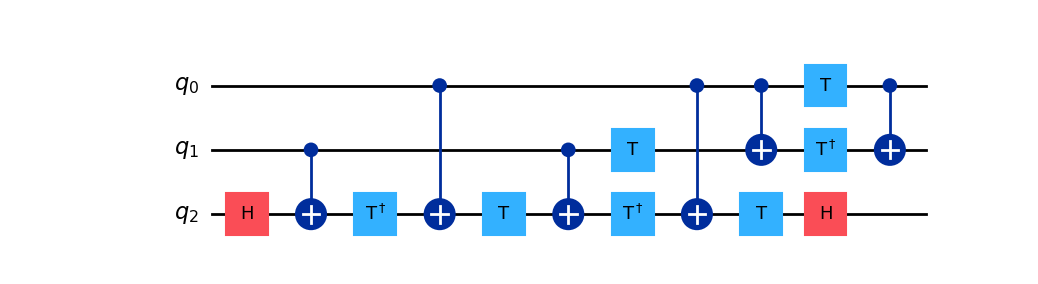
\includegraphics[width=0.8\textwidth]{Figures/toffoli_def.png} 
    \caption{Toffoli definition} 
    \label{fig:toffoli_def} 
\end{figure}
\subsubsection{Simplified Toffoli}
Aside from the definition of a Toffoli gate given by Figure \ref{fig:toffoli_def} we can utilize the simplified Toffoli gate also known as the Margolis gate \cite{barenco_elementary_1995} illustrated in Figure \ref{fig:rccx},  which was shown to be optimal for a single Toffoli gate \cite{song2003simplifiedtoffoligateimplementation} with a minimum of 3 Cnots and 4 single qubit gates.
\begin{figure}[H] 
    \centering 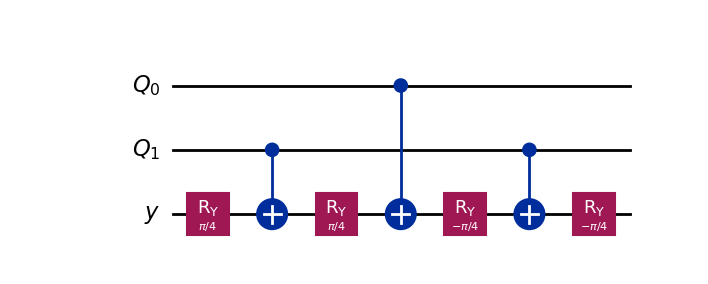
\includegraphics[width=0.8\textwidth]{Figures/rccx.png} 
    \caption{Margolis Gate} 
    \label{fig:rccx} 
\end{figure}
We are able to simplify this further since the computational basis is not impacted by relative phase. 
When multiple Margolis gates act sequentially together we can further reduce the gate number by combining redundant gates as suggested in this blogpost \cite{patrick_downing_qiskit_2021}.\begin{figure}[H] 
    \centering 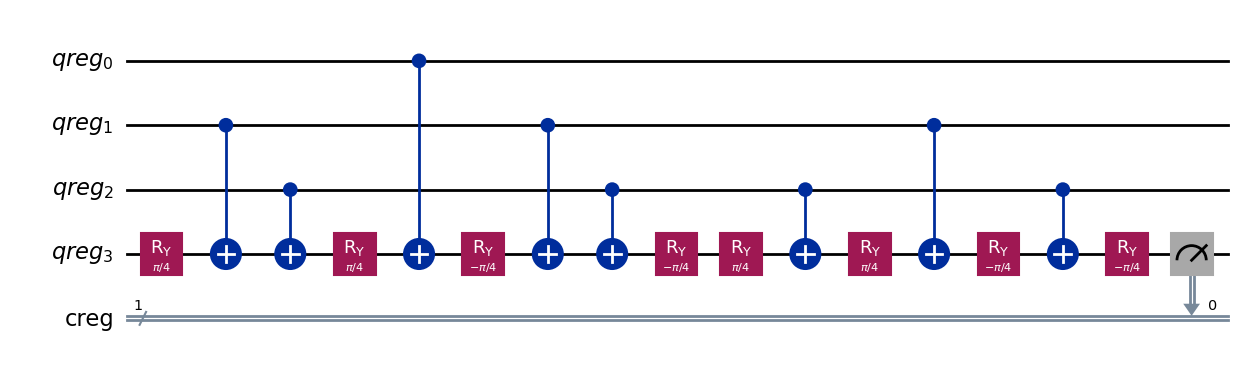
\includegraphics[width=0.6\textwidth]{Figures/intermediate_margolis.png} 
    \caption{Combining two margolis gates} 
    \label{fig:2margolis} 
\end{figure}
\begin{figure}[H] 
    \centering 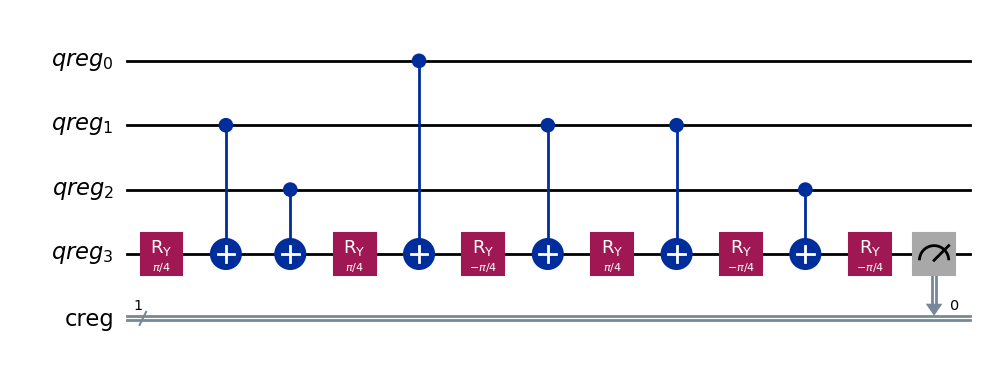
\includegraphics[width=0.8\textwidth]{Figures/n3j2_margolis_compact.png} 
    \caption{Simplified circuit diagram for \(n=3, j=2\) popcount problem} 
    \label{fig:simplified_margolis} 
\end{figure}
Since \(Toffoli(q_0,q_1,q_3)\) \& \(Toffoli(q_0,q_2,q_3)\) both involve \(q_0\) as a control bit, instead of recomputing the operations for \(q_0\) we can instead add two \(Cnot(q_2,q_3)\) into \(Toffoli(q_0,q_1,q_3)\) as shown in Figure \ref{fig:2margolis}.
As we can see the two central \(Cnot(q_2,q_3)\) and \(R_y\) gates cancel out allowing us to remove them giving us the resulting circuit illustrated in Figure \ref{fig:simplified_margolis}. To verify this solution for the \(j=2,n=3\) problem we used Qiskit to simulate the circuit. The code can be examined in appendix\ref{appendix_a}, except the \texttt{\textbf{create\_QPE\_popcount\_circuit\_rcx()}}
 is exchanged for \ref{compact_margolis_solution_code}.


\subsubsection{Generalizing the Exhaustive Toffoli approach to \( n \ge 2\)}

We can clearly see a pattern in the specific solutions for the \(n=3\) and \(n=4\) problem instances. In both cases all possible combinations of input qubit pairs are covered by one Toffoli gate. The number of Toffoli gates is given by the binomial coefficient \(\binom{n}{2}\) each time: \(\binom{3}{2} = 3, \binom{4}{2} = 6\). An obvious question is thus if this approach can be used for any \(n \in \mathbb{N}\) with \(j=2\).

To answer that question we can analyse how the \(y_2\) output bit behaves for any \(\omega(z) \in \mathbb{N}\) value. The \(y_2\) qubit is the second least significant bit in a binary number. The decimal value that this bit corresponds to when set to 1 is 2. If it is set to 0, it is 0 in decimal value. The contribution from this bit can be interpreted as periodic starting from \(0_{10}\) with a period of \(4_{10}\) where the bit is set to 0 in the first two cases and 1 in the last two. For \(y_1\) we showed that the circuit generalizes because the circuit flips the output qubit only if the number of activated CNOTs is odd. This could be expressed with modular arithmetic where we use that the decimal value is divisible by 2 (even) if the bit should be 0 and not divisible by 2 (odd) if it should be 1:

\[\ket{z_n, y_2} = \ket{z_n} \otimes X^{\omega(z_n) \; mod \; 2}\ket{0}\]

The general circuit for \(j=2\) should therefore implement a function that given the number of set bits \(\omega(z)\) gives an output alternating between two odd decimal values and two even integer numbers. If we now look at the binomial coefficient which determines the number of times the X gate is applied to \(y_2\) and the cases where \(k=2\), we can see that exactly that pattern of even and odd integers occur in the output.

\[\binom{n}{k} = \frac{\prod^{n}_{i = n-k}i}{k!}\]

For \(k=2\) we can observe that the numerator consists of the two factors \(n-1\) and \(n\). Every other integer in the lexicographically ordered \(\mathbb{Z}\) must be an even number, thus there is always at least one occurrence of the factor 2 in the numerator. So for all n such that \(n\) or \(n-1\) only contains one factor 2, the result will be an odd number. In all other cases the, coefficient is even. The binomial coefficient is in other words even every time \(n\) or \(n-1\) is a multiple of \(4 = 2 \cdot 2\). A multiple of 4 occurs each \(4\)-th integer in the lexicographic ordered series of integers. Every such integer also accounts for two even binomial coefficients: once for when it is equal to \(n\) and once for when it is equal to \(n-1\). 

We can illustrate this by looking at the first four integers. The first integer is 2, which is not a multiple of 4 and results in an odd binomial coefficient. The same applies to \(n=3\). The next two are even as the first multiple is reached for \(n=4\) and for \(n=5\) we have \(n-1 = 4\). Note that the binomial coefficient \(\binom{n}{2}\) is not defined for \(n \in \{0,1\}\), which is fine because for those cases the \(y_2\) output bit is not defined. It is therefore clear that the binomial coefficient provides the output pattern we are looking for to express the function in modular arithmetic like for \(y_1\). We can write:

\[y_2 = \binom{\omega(z_n)}{2} \; mod \; 2\]

Since the number of activated Tofflo gates in the Exhaustive Toffoli circuit, we can express the effect of the circuit \(ET_n\) for any \(n \ge 2\) like this:

\[\ket{z_n, y_2} \xrightarrow{ET} 
    \begin{cases}
    \ket{z_n, 0} & 2 > \omega(z_n) \ge 0 \\
    \ket{z_n} \otimes X^{\binom{\omega(z_n)}{2}}\ket{0} & \omega(z_n) \ge 2
    \end{cases}
\]

\subsubsection{Finding \(y_2\)  with the Quantum Fourier Transform}
From the previous section we know that using the ET circuit does generalize to all \(n \ge 2\) for the \(j=2\) problem configuration. Another approach to solve the popcount problem on a Quantum Computer can be found in \cite{mit_problem_set_2010}. In this case they used the Quantum Fourier Transform (QFT) to solve the problem for any \(n \in \mathbb{N}\) for all \(y_j\). This is thus an interesting starting point to create a general solution for the problem configuration \(n \ge 2\) with \(j = 2\). Table 4 shows the general circuit with:

\begin{table}[h!]
\centering

\Qcircuit @C=0.7em @R=1.6em {
    \lstick{} & \ket{z_1}         & & \qw                & \ctrl{3}   & \qw & \hdots & & \qw        & \qw & \ctrl{4}   & \qw & \hdots & &\qw         & \qw & \ctrl{6}   & \qw & \hdots & & \qw        & \qw & \qw                     & \qw                                    & &\\
    \lstick{} & \vdots \notag     & &                    &            &     &        & &            &     &            &     &        & &            &     &            &     &        & &            &     &                         &                                        & &\ket{z} \\
    \lstick{} & \ket{z_n}         & & \qw                & \qw        & \qw & \hdots & & \ctrl{1}   & \qw & \qw        & \qw & \hdots & & \ctrl{2}   & \qw & \qw        & \qw & \hdots & & \ctrl{4}   & \qw & \qw                     & \qw \gategroup{1}{24}{3}{24}{1em}{\}} & &
        \inputgroupv{1}{3}{1em}{1.7em}{\ket{z}\quad} \\
    \lstick{} & \ket{0}           & & \multigate{3}{QFT} & \gate{R_1} & \qw & \hdots & & \gate{R_1} & \qw & \qw        & \qw & \hdots & & \qw        & \qw & \qw        & \qw & \hdots & & \qw        & \qw & \multigate{3}{QFT^{-1}} & \qw                                    & &\\
    \lstick{} & \ket{0}           & & \ghost{QFT}        & \qw        & \qw & \hdots & & \qw        & \qw & \gate{R_2} & \qw & \hdots & & \gate{R_2} & \qw & \qw        & \qw & \hdots & & \qw        & \qw & \ghost{QFT^{-1}}        & \qw                                    & & \quad \quad \ket{\omega(z)}\\
    \lstick{} & \vdots \notag     & &                    &            &     &        & &            &     &            &     &        & &            &     &            &     &        & &            &     &                         &                                        & &\\
    \lstick{} & \ket{0}           & & \ghost{QFT}        & \qw        & \qw & \hdots & & \qw        & \qw & \qw        & \qw & \hdots & & \qw        & \qw & \gate{R_m} & \qw & \hdots & & \gate{R_m} & \qw & \ghost{QFT^{-1}}        & \qw \gategroup{4}{24}{7}{24}{1em}{\}} & &  
        \inputgroupv{4}{7}{1em}{3.8em}{\ket{0^{\otimes m}}\quad} \\
}

\caption{The solution presented by \cite{mit_problem_set_2010}}
\label{table:mit_solution}
\end{table}



\[
    R_k = 
    \begin{bmatrix}
        1 & 0 \\
        0 & e^{2\pi i/2^k}
    \end{bmatrix}
\]

One problem with this solution is that it uses m qubits to represent the output. In our case, we are limited to using one qubit (qubit constraint). However, the QFT algorithm depends on access to the less significant bits of the most significant bit. This can be observed from the definition of the QFT \cite[p. 363]{sutor_dancing_2019}: 
\[
    QFT_n(\ket{\varphi}) = \frac{1}{\sqrt{2^n}} \sum^{2^n-1}_{j=0} \sum^{2^n-1}_{k=0} a_k e^\frac{2 \pi i j k}{2^n} \ket{j}_n
\]

Where \(n\) is the number of input bits and \(\ket{\varphi} = \frac{1}{\sqrt{2^n}} \sum^{2^n-1}_{j=0} a_j \ket{j}_n\). The phase of each input configuration \(j\) is the sum of the amplitudes \(a_k\) from the input state times \(e^\frac{2 \pi i j k}{2^n}\). In the exponent \(\frac{2 \pi i j k}{2^n}\) the value of j (current standard basis) determines the phase. Thus the phase of the output depends on the value of the input. To find the correct phase of each qubit, the algorithm needs information from the other qubits. One can better observe this in the circuit diagram (see Figure \ref{fig:qft_3}) where it is clear that the less significant bit controls the phase shift of all the more significant bits. 

Another important observation is that the input state of the input to the QFT is \(\ket{0}^{\otimes m}\). Since all the controlled operators only effect the circuit for the \(\ket{1}\) state, only the \(H^{\otimes m}\) is applied, resulting in a state \(\frac{1}{2^n} \sum^{2^n-1}_{j=0} \ket{j}\). It is therefore only the \(QFT^{-1}\) where the dependency is for the less significant bits lies. 

\begin{figure}[htbp] 
    \centering 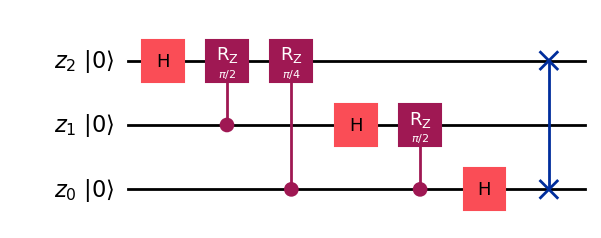
\includegraphics[width=1\textwidth]{Figures/qft_3_figure.png} 
    \caption{The circuit diagram for $QFT_3$} 
    \label{fig:qft_3} 
\end{figure}

\begin{figure}[htbp] 
    \centering 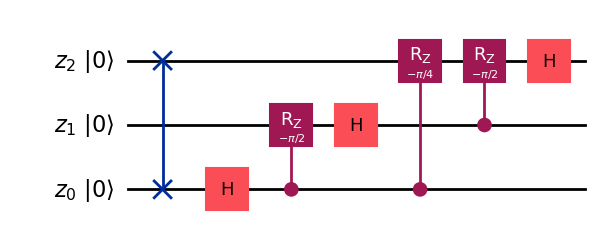
\includegraphics[width=1\textwidth]{Figures/inverse_qft_3.png} 
    \caption{The circuit diagram for ${QFT^{-1}}_3$} 
    \label{fig:inv_qft_3} 
\end{figure}

When explicitly looking at the \(j=2\) case, the \(QFT^{-1}\) is only depending on the least significant bit \(y_{j=1}\). It is also important to note that we can change the state of the \(n\) input bits after the \(CR_z\) gates have been applied, because the needed information is encoded into \(y_{j=2}\) by that point. The question is thus if it is possible to obtain the state of \(y_{j=1}\) with the \(n\) qubits. 

Looking at the solutions for \(j=1\) problems, we see the pattern of applying the X gate to the \(y_{j=1}\) qubit as many times as there are \(\ket{1}\) qubits in the input. This is done by applying \(n\) CNOT gates where each input is set to be control bit to one of them and the target is always the \(y_{j=1}\) qubit. If we now reduce the number of CNOT gates by one and set one of the inputs to be the target qibut for all the CNOT gates without being a control qubit for any of the CNOT gates. Since this input qubit is either \(\ket{0}\) or \(\ket{1}\), setting the input to \(\ket{1}\) will be the equivalent of applying the X gate once more. Thus we have a solution to the \(j=1\) configuration with \(n\) qubits used and \(n-1\) CNOT gates used. With the \(y_{j=1}\) information encoded in another qubit, we are able to apply the controlled \(S^{\dagger}\) gate (i.e. \(CR_z(-\frac{\pi}{2})\)) with control bit set to the \(y_{j=1}\) and the target being the \(y_{j=2}\) qubit. What remains of the \(QFT^{-1}_{2}\) algorithm is to change the bit back to the \(\ket{0}, \ket{1}\) basis with the Hadamard gate. The described solution is presented as a circuit in Figure \ref{fig:general_qft_solution}.

\begin{figure}[t] 
    \centering 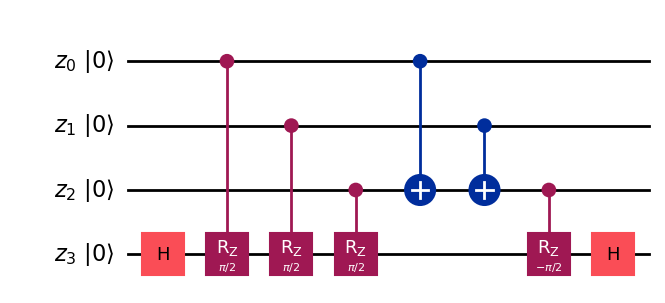
\includegraphics[width=1\textwidth]{Figures/qft_solution_j2_rz.png} 
    \caption{The circuit diagram for the QFT solution to n=3 j=2 popcount problem} 
    \label{fig:qft_rz_solution} 
\end{figure}

\begin{figure}[t]
\centering
\Qcircuit @C=0.7em @R=1.6em {
    \lstick{} & & \ket{z_1}         &  & & \qw           & \ctrl{5}           & \qw                & \qw & \; \hdots \notag \; & & \qw                & \qw                & \ctrl{4} & \qw      & \qw & \; \hdots \notag \; &     & \qw      & \qw                 & \qw      & \qw & \\
    \lstick{} & & \ket{z_2}         &  & & \qw           & \qw                & \ctrl{4}           & \qw & \; \hdots \notag \; & & \qw                & \qw                & \qw      & \ctrl{3} & \qw & \; \hdots \notag \; &     & \qw      & \qw                 & \qw      & \qw & \\
    \lstick{} & & \vdots \notag     &  & &               &                    &                    &     &                     & &                    &                    &          &          &     &                     &     &          &                     &          &     & \\
    \lstick{} & & \ket{z_{n-1}}     &  & & \qw           & \qw                & \qw                & \qw & \; \hdots \notag \; & & \ctrl{2}           & \qw                & \qw      & \qw      & \qw & \; \hdots \notag \; &     & \ctrl{1} & \qw                 & \qw      & \qw & \\
    \lstick{} & & \ket{z_n}         &  & & \qw           & \qw                & \qw                & \qw & \; \hdots \notag \; & & \qw                & \ctrl{1}           & \targ    & \targ    & \qw & \; \hdots \notag \; &     & \targ    & \ctrl{1}            & \qw      & \qw &
        \inputgroupv{1}{5}{1em}{3.7em}{\ket{z}\quad} \\
    y_2       & & \ket{0}           &  & & \gate{H}      & \gate{R_z^{\pi/2}} & \gate{R_z^{\pi/2}} & \qw & \; \hdots \notag \; & & \gate{R_z^{\pi/2}} & \gate{R_z^{\pi/2}} & \qw      & \qw      & \qw & \; \hdots \notag \; &     & \qw      & \gate{R_z^{-\pi/2}} & \gate{H} & \qw & \\
}


\caption{The general solution to the \(j=2\) popcount problem}
\label{fig:general_qft_solution}
\end{figure} 

Another limitation is that we can only use the CNOT operator and any single qubit operators. The \(CR_z\) gate needs therefore to be decomposed for this solution to be valid. Finding a decomposition that is exact is however difficult. The matrix of the \(CR_z\) gate is known \cite[p. 293]{sutor_dancing_2019}:

\[
    CR_z(\varphi) = 
    \begin{bmatrix}
        1 & 0 & 0 & 0 \\
        0 & 1 & 0 & 0 \\
        0 & 0 & 1 & 0 \\
        0 & 0 & 0 & e^{\varphi i}
    \end{bmatrix}
\]

It was difficult to find a circuit that matches that transformation. One example is the decomposition mentioned in \cite{liu_analysis_2024} (see \ref{fig:crz_decomp}). That approach produces a slightly different matrix. The matrix for the circuit can be found by doing the following calculation:

\begin{figure}[t] 
    \centering 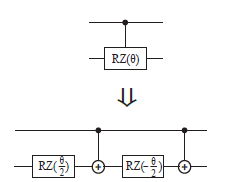
\includegraphics[width=0.4\textwidth]{Figures/crz_decomposition.png} 
    \caption{The crz decomposition from \cite{liu_analysis_2024}}
    \label{fig:crz_decomp} 
\end{figure}

\[
CR_z(\varphi)' = \left(I_2 \otimes R_z\left(\frac{\varphi}{2}\right)\right) \cdot CNOT \cdot \left(I_2 \otimes R_z\left(-\frac{\varphi}{2}\right)\right) \cdot CNOT \]
\[
= 
    \begin{bmatrix}
        1 & 0 & 0 & 0 \\
        0 & e^{\frac{\varphi}{2} i} & 0 & 0 \\
        0 & 0 & 1 & 0 \\
        0 & 0 & 0 & e^{\frac{\varphi}{2} i}
    \end{bmatrix}
    \begin{bmatrix}
        1 & 0 & 0 & 0 \\
        0 & 1 & 0 & 0 \\
        0 & 0 & 0 & 1 \\
        0 & 0 & 1 & 0
    \end{bmatrix}
    \begin{bmatrix}
        1 & 0 & 0 & 0 \\
        0 & e^{-\frac{\varphi}{2} i} & 0 & 0 \\
        0 & 0 & 1 & 0 \\
        0 & 0 & 0 & e^{-\frac{\varphi}{2} i}
    \end{bmatrix}
    \begin{bmatrix}
        1 & 0 & 0 & 0 \\
        0 & 1 & 0 & 0 \\
        0 & 0 & 0 & 1 \\
        0 & 0 & 1 & 0
    \end{bmatrix} \]
    \[
    = 
        \begin{bmatrix}
        1 & 0 & 0 & 0 \\
        0 & e^{\frac{\varphi}{2} i} & 0 & 0 \\
        0 & 0 & 0 & 1 \\
        0 & 0 & e^{\frac{\varphi}{2} i} & 0
    \end{bmatrix}
    \begin{bmatrix}
        1 & 0 & 0 & 0 \\
        0 & e^{-\frac{\varphi}{2} i} & 0 & 0 \\
        0 & 0 & 1 & 0 \\
        0 & 0 & 0 & e^{-\frac{\varphi}{2} i}
    \end{bmatrix}
    \begin{bmatrix}
        1 & 0 & 0 & 0 \\
        0 & 1 & 0 & 0 \\
        0 & 0 & 0 & 1 \\
        0 & 0 & 1 & 0
    \end{bmatrix} \]
    \[
    = 
    \begin{bmatrix}
        1 & 0 & 0 & 0 \\
        0 & 1 & 0 & 0 \\
        0 & 0 & 0 & e^{-\frac{\varphi}{2} i} \\
        0 & 0 & e^{\frac{\varphi}{2} i} & 0
    \end{bmatrix}
    \begin{bmatrix}
        1 & 0 & 0 & 0 \\
        0 & 1 & 0 & 0 \\
        0 & 0 & 0 & 1 \\
        0 & 0 & 1 & 0
    \end{bmatrix} 
    \]
    \[
    = 
    \begin{bmatrix}
        1 & 0 & 0 & 0 \\
        0 & 1 & 0 & 0 \\
        0 & 0 & e^{-\frac{\varphi}{2} i}  & 0\\
        0 & 0 & 0 & e^{\frac{\varphi}{2} i}
    \end{bmatrix}
\]
From the matrices, we can see that the operations only affect the target qubit with the \(2\times2\) matrix in the lower right corner. The difference is that \(CR_z(\varphi)'\), in addition to state \(\ket{11}\) also has an effect on the \(\ket{10}\) state. The lower right \(2\times2\) matrices for \(CR_z(\varphi)\) and \(CR_z(\varphi)'\), are representations of the \(R_z(\varphi)\) single qubit gate with a difference of a complex factor \(e^{\frac{\varphi}{2}i}\) \cite[p. 261]{sutor_dancing_2019}:
\[
\begin{bmatrix}
1 & 0 \\
0 & e^{\varphi i}
\end{bmatrix} 
= e^{\frac{\varphi}{2}i}
\begin{bmatrix}
e^{-\frac{\varphi}{2}i} & 0 \\
0 & e^{\frac{\varphi}{2}i}
\end{bmatrix} 
\]
This common factor is a complex number with an absolute value of \(1\) and does not affect the amplitudes of the basis states. The difference should therefore not have an effect in this case. This can be observed by analysing how the two operations are applied to a qubit in the \(\ket{+}\) state:

\[
    \begin{bmatrix}
1 & 0 \\
0 & e^{\varphi i}
\end{bmatrix} \left(\frac{\ket{0} + \ket{1}}{\sqrt{2}}\right)
= \frac{1}{\sqrt{2}}\left(
 \begin{bmatrix}
1 & 0 \\
0 & e^{\varphi i}
\end{bmatrix}
 \begin{bmatrix}
1 \\
0 
\end{bmatrix}
+ \begin{bmatrix}
1 & 0 \\
0 & e^{\varphi i}
\end{bmatrix}
 \begin{bmatrix}
0 \\
1 
\end{bmatrix}\right)
= \frac{1}{\sqrt{2}}\ket{0} + \frac{e^{\varphi i}}{\sqrt{2}}\ket{1}
\]
If we now do the same calculation with the decomposed matrix, we can see that the relative phase is equal \cite[p. 248-249]{sutor_dancing_2019}:
\[
    \begin{bmatrix}
e^{-\frac{\varphi}{2} i} & 0 \\
0 & e^{\frac{\varphi}{2} i}
\end{bmatrix} \left(\frac{\ket{0} + \ket{1}}{\sqrt{2}}\right)
= \frac{1}{\sqrt{2}}\left(
 \begin{bmatrix}
e^{-\frac{\varphi}{2} i} & 0 \\
0 & e^{\frac{\varphi}{2} i}
\end{bmatrix}
 \begin{bmatrix}
1 \\
0 
\end{bmatrix}
+ \begin{bmatrix}
e^{-\frac{\varphi}{2} i} & 0 \\
0 & e^{\frac{\varphi}{2} i}
\end{bmatrix}
 \begin{bmatrix}
0 \\
1 
\end{bmatrix}\right)
= \frac{e^{-\frac{\varphi}{2} i}}{\sqrt{2}}\ket{0} + \frac{e^{\frac{\varphi}{2} i}}{\sqrt{2}}\ket{1} 
\]
\[
= e^{-\frac{\varphi}{2} i} \left(\frac{1}{\sqrt{2}}\ket{0} + \frac{e^{\left(\frac{\varphi}{2} + \frac{\varphi}{2}\right) i}}{\sqrt{2}}\ket{1}\right)\;,\;\; where \;\; \varphi = \frac{\varphi}{2}+\frac{\varphi}{2}
\]



When using the decomposition mentioned above we can see that the operation performed on the target is given by the following matrix:
\[
    S' = CR_z(\pi/2) = \begin{bmatrix}
        e^{-\frac{\pi}{4} i}  & 0\\
        0 & e^{\frac{\pi}{4} i}
    \end{bmatrix}
\]
Now we can substitute \(S'\) into the function expression and use that it is a diagonal matrix:
\[
    (S')^{\omega(z)-y_1} = 
    \begin{bmatrix}
        e^{-\frac{\pi}{4} i(\omega(z)-y_1)}  & 0\\
        0 & e^{\frac{\pi}{4} i(\omega(z)-y_1)}
    \end{bmatrix}
\]
The target qubit starts in the \(\ket{0}\) state and is transformed into the \(\ket{+}\) state after the first Hadamard gate. Next the \(S'\) operators are applied (note that the inverse S gate is applied by subtracting the exponent with \(y_1\)):
\[
(S')^{\omega(z)-y_1}\ket{0} =     \begin{bmatrix}
        e^{-\frac{\pi}{4} i(\omega(z)-y_1)}  & 0\\
        0 & e^{\frac{\pi}{4} i(\omega(z)-y_1)}
    \end{bmatrix} 
    \begin{bmatrix}
        1 \\
        0
    \end{bmatrix} = \begin{bmatrix}
         e^{-\frac{\pi}{4} i(\omega(z)-y_1)}\\
        0
    \end{bmatrix} = e^{-\frac{\pi}{4} i(\omega(z)-y_1)}\ket{0}
\]
\[
(S')^{\omega(z)-y_1}\ket{1} =     \begin{bmatrix}
        e^{-\frac{\pi}{4} i(\omega(z)-y_1)}  & 0\\
        0 & e^{\frac{\pi}{4} i(\omega(z)-y_1)}
    \end{bmatrix} 
    \begin{bmatrix}
        0 \\
        1
    \end{bmatrix} = \begin{bmatrix}
         0\\
        e^{\frac{\pi}{4} i(\omega(z)-y_1)}
    \end{bmatrix} = e^{\frac{\pi}{4} i(\omega(z)-y_1)}\ket{1}
\]
With that we can find:
\[
    (S')^{\omega(z)-y_1}\ket{+} = \frac{\left((S')^{\omega(z)-y_1}\ket{1} + (S')^{\omega(z)-y_1}\ket{0}\right)}{\sqrt{2}} 
    \]
    
\[
=\frac{e^{-\frac{\pi}{4} i(\omega(z)-y_1)}\ket{0} + e^{\frac{\pi}{4} i(\omega(z)-y_1)}\ket{1}}{\sqrt{2}} \;\; \underrightarrow{H} \;\; \frac{e^{-\frac{\pi}{4} i(\omega(z)-y_1)}H\ket{0} + e^{\frac{\pi}{4} i(\omega(z)-y_1)}H\ket{1}}{\sqrt{2}}
\]
\[
     = \frac{e^{-\frac{\pi}{4} i(\omega(z)-y_1)}(\ket{0} + \ket{1}) + e^{\frac{\pi}{4} i(\omega(z)-y_1)}(\ket{0} - \ket{1})}{\sqrt{2}^2} 
\]
\[
    = \frac{\ket{0} \left(e^{-\frac{\pi}{4} i(\omega(z)-y_1)} + e^{\frac{\pi}{4} i(\omega(z)-y_1)}\right)+ \ket{1}\left(  e^{-\frac{\pi}{4} i(\omega(z)-y_1)} - e^{\frac{\pi}{4} i(\omega(z)-y_1)}  \right)}{2}
\]
The amplitudes for the two standard basis have now been separated and we can calculate the probability of measuring each of the states: 

\[
p_\ket{0} = \left|\frac{e^{-\frac{\pi}{4} i(\omega(z)-y_1)} + e^{\frac{\pi}{4} i(\omega(z)-y_1)}}{2}\right|^2
\]

\[
p_\ket{1} = \left|\frac{e^{-\frac{\pi}{4} i(\omega(z)-y_1)} - e^{\frac{\pi}{4} i(\omega(z)-y_1)}}{2}\right|^2
\]

where
\[
    e^{-\frac{\pi}{4} i(\omega(z)-y_1)} = cos(-\frac{\pi}{4}\cdot(\omega(z) - y_1)) + sin(-\frac{\pi}{4}\cdot(\omega(z) - y_1))i
\]
\[
    = cos(\frac{\pi}{4}\cdot(\omega(z) - y_1))  - sin(\frac{\pi}{4}\cdot(\omega(z) - y_1))i
\]
\[
    e^{\frac{\pi}{4} i(\omega(z)-y_1)} = cos(\frac{\pi}{4}\cdot(\omega(z) - y_1)) + sin(\frac{\pi}{4}\cdot(\omega(z) - y_1))i \]
\[
    = cos(\frac{\pi}{4}\cdot(\omega(z) - y_1))  + sin(\frac{\pi}{4}\cdot(\omega(z) - y_1))i
\]
We can identify two common terms: \(a := cos(\frac{\pi}{4}\cdot(\omega(z) - y_1))\) and \(b := sin(\frac{\pi}{4}\cdot(\omega(z) - y_1))\). With that we can rewrite:

\[
    e^{-\frac{\pi}{4} i(\omega(z)-y_1)} + e^{\frac{\pi}{4} i(\omega(z)-y_1)} = a-bi + a + bi = 2a
\]
\[
    e^{-\frac{\pi}{4} i(\omega(z)-y_1)} - e^{\frac{\pi}{4} i(\omega(z)-y_1)} = a - bi - (a + bi) = a -a -bi -bi = -2bi
\]
The probabilities can now be simplified
\[
    p_\ket{0}= \left|\frac{2a}{2}\right|^2 = \left|cos\left(\frac{\pi}{4}\cdot(\omega(z) - y_1)\right)\right|^2
\]
\[
    p_\ket{1}= \left|\frac{-2bi}{2}\right|^2 =|b|^2= \left|sin\left(\frac{\pi}{4}\cdot(\omega(z) - y_1)\right)\right|^2
\]
We see that the measured result depends on the periodic trigonometric functions. Because they are periodic, we primarily need to concider the the cases where the angle is between 0 and \(2\pi\). 
\[
    \frac{\pi}{4} \cdot x = 2\pi \Leftrightarrow x = \frac{2\pi \cdot 4}{\pi} = 8
\]
We can now examine the effect of the circuit with a truth table where all possible cases within the first period is listed. Those cases are the 8 first possible function values of \(\omega(z) \in \{a \in \mathbb{Z}|0 \le a < 8\}\) (see table \ref{table:qft_truth}). From the table we can observe that the state of the qubit, always ends up in a deterministic state that matches the expected values of \(y_2\). From this we can see that the QFT solution can be applied to \(j=2\) popcount problem with \(n \ge 2\).

\begin{table}[t]
\caption{The truth table for the QFT solution for the \(j=2\) popcount problem. The truth table contains all special cases within the first period}
\label{table:qft_truth}
\begin{center}
\begin{tabular}{|c |c |c |c|c|c|} 
 \hline
 \(\omega(z)\)& $y_1$ & expected $y_2$ & $\frac{\pi}{4}\cdot(\omega(z) - y_1)$ & $p_\ket{0}$ & $p_\ket{1}$\\  
 \hline\hline
 0& 0& 0& 0&  $\left|cos\left(0\right)\right|^2 = 1$&$\left|sin\left(0\right)\right|^2 = 0$\\ 
 \hline
 1& 1& 0& $\frac{\pi}{4} (1 -1) = 0$& $\left|cos\left(0\right)\right|^2 = 1$&$\left|sin\left(0\right)\right|^2 = 0$\\
 \hline
 2& 0& 1& $\frac{\pi}{4} (2 -0) = \frac{\pi}{2}$& $\left|cos\left(\frac{\pi}{2}\right)\right|^2 = 0$&$\left|sin\left(\frac{\pi}{2}\right)\right|^2 = 1$\\
 \hline
 3& 1& 1& $\frac{\pi}{4} (3 - 1) = \frac{\pi}{2}$& $\left|cos\left(\frac{\pi}{2}\right)\right|^2 = 0$&$\left|sin\left(\frac{\pi}{2}\right)\right|^2 = 1$\\
 \hline
 4& 0& 0& $\frac{\pi}{4} (4 -0) = \pi$& $\left|cos(\pi)\right|^2 = 1$&$\left|sin(\pi)\right|^2 = 0$\\ 
 \hline
 5& 1& 0& $\frac{\pi}{4} (5 - 1) = \pi$& $\left|cos(\pi)\right|^2 = 1$&$\left|sin(\pi)\right|^2 = 0$\\ \hline 
 6& 0& 1& $\frac{\pi}{4} (6 - 0) = \frac{3\pi}{2}$& $\left|cos\left(\frac{3\pi}{2}\right)\right|^2 = 0$&$\left|sin\left(\frac{3\pi}{2}\right)\right|^2 = 1$\\ \hline 
 7& 1& 1& $\frac{\pi}{4} (7 - 1) = \frac{3\pi}{2}$& $\left|cos\left(\frac{3\pi}{2}\right)\right|^2 = 0$&$\left|sin\left(\frac{3\pi}{2}\right)\right|^2 = 1$\\\hline
\end{tabular}
\end{center}
\end{table}

\begin{figure}[htbp] 
    \centering 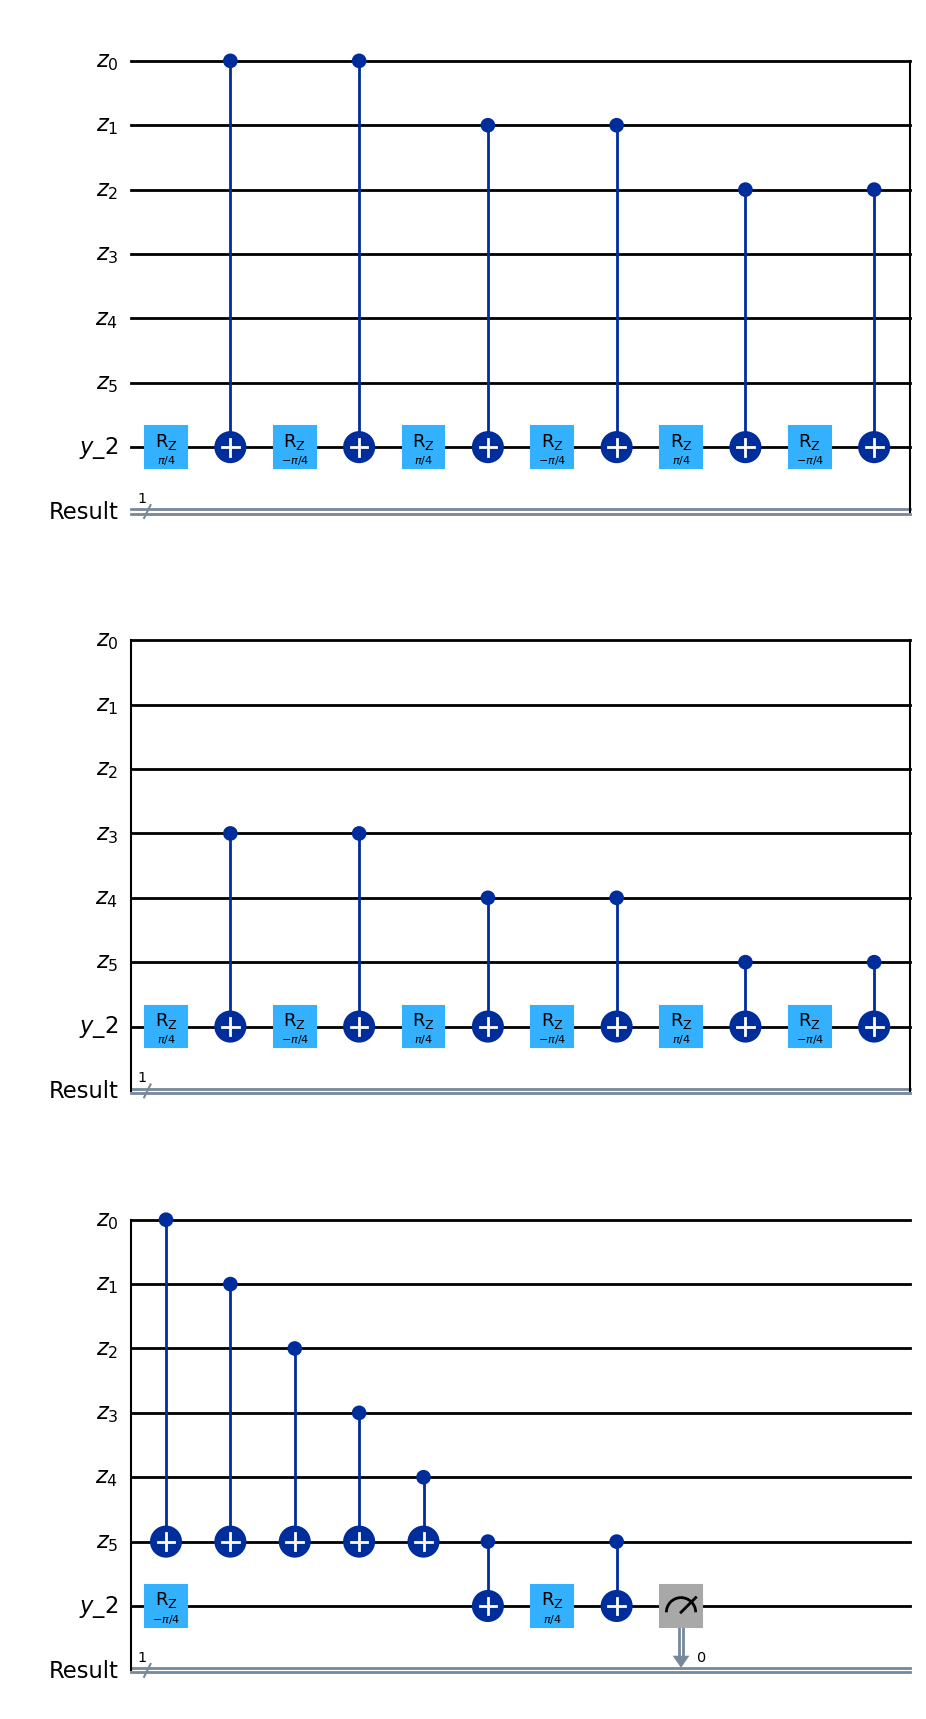
\includegraphics[width=0.8\textwidth]{Figures/QFT_decomposed_solution_n=6.png} 
    \caption{Circuit diagram for \(n=6\), \(j=2\) with \(CR_z\) decomposition.} 
    \label{fig:qft_crz_circuit_drawing} 
\end{figure}   

To verify this solution for the \(j=2, n=6\) problem instance, we used Qiskit to simulate the circuit (see Figure 14). The code can be reviewed in \nameref{appendix_a}.


\subsubsection{Comparing the two solutions}

Since we have found two different circuits that can be used to solve the \(j=2\) popcount problem, it is interesting to compare them in how efficient they are solving the problem. The number of gates needed with regards to the number of input bits, is a metric that can be used to get insight on how effective the algorithms are. It is also interesting to count the number of specific gates since some gates are more expensive in the amount of resources needed. In \cite{lee_cost_2006} it is shown that the CNOT gate has a cost that is 5 times that of the X gate on an ideal Quantum Computer. 

From the analysis about the Exhaustive Toffoli approach we know that the number of Toffoli gates is given by the binomial coefficient. Furthermore, the Toffoli gate can be decomposed by using 6 CNOT gates and 9 single qubit gates.

Number of CNOT gates:
\[
    N_{CNOT} = \binom{n}{2}\cdot 6 = \frac{6n(n-1)}{2} = 3(n^2 - n) = O(n^2)
\]
Total number of gates:
\[
    N_{total} = \binom{n}{2}\cdot 15 = \frac{15n(n-1)}{2} = \frac{15}{2}(n^2 - n) = O(n^2)
\]

For the QFT solution tot he \(j=2\) popcount problem, we can count the number of CRZ gates as n (each input corresponds to one CRZ gate). furthermore there are two Hadamard gates and one CRZ gate in the \(QFT\) and \(QFT^-1\). The CRZ gate can be decomposed into two RZ gates and two CNOT gates.

Number of CNOT gates:
\[
N_{CNOT} = 2 + n\cdot2 = O(n)
\]
Total number of gates:
\[
N_{total} = 6 + 4n + n - 1 = O(n)
\]

From this we see that the QFT solution is significantly less costly as it is done with a linear amount of gates compared to the Toffoli approach where the number of gates grows quadratically. 

\subsection{Solution to the \(j=3\) popcount problem}

To solve the \(j=3\) popcount problem, we can use the same thought process as for the Exhaustive Toffoli approach \(j=2\) where all possible input pairs are used as control bits for a unique Toffoli gate. We were able to show that this approach generalizes to problems with any input size because the binomial coefficient with \(k=2\) produces two odd and two even numbers periodically when \(\omega(z)\) increases. 

\begin{figure}[t]
    \centering
    \Qcircuit @C=0.7em @R=1.6em {
         & \qw & \ctrl{4} & \qw & & \\
         & \qw & \ctrl{3} & \qw & & \\
         & \qw & \ctrl{2} & \qw & & \\
         & \qw & \ctrl{1} & \qw & & \\
         & \qw & \targ & \qw & & \\
    }
    
\caption{A five qubit gate which is applying the X gate on a target if four control qubits are in state \(\ket{1}\).}
\label{fig:quad_cnot}
\end{figure}

The expected output \(y_3\) can be observed to be zero for four values and one for four subsequent values when we iterate over the lexicographically ordered sequence of Integers for \(\omega(z)\). In other words we need a circuit that produces four even numbers sequentially and four odd numbers sequentially such that the X gate is canceled out for the four even numbers and applied once for the odd numbers. 

If we would be to create a gate that is controlled by four qubits, we would be able to find \(\binom{n}{4}\) different input combinations. The number of times the X gate is applied is thus also given by \(\binom{\omega(z)}{4}\) where \(\omega(z), n \ge 4\). By using the same reasoning as for the \(j=2\) problem instance, we can observe that the binomial coefficient produces first four even numbers and then four odd numbers and repeats this pattern periodically if we sequentially calculate it for the lexicographically ordered set of positive integers greater than 4. 
\[
\binom{\omega}{4} = \frac{\omega(\omega - 1)(\omega - 2)(\omega - 3)}{4!}
\]
The numerator consists of four factors which form a sequence of difference 1. The denominator contains three factors of 2: \(4! = 4\cdot3\cdot2\cdot1 = 2^3\cdot3\). In the cases where the four factors in the denominator contain only 3 factors of two, the result will be odd. If there are four factors of two \(2^4 = 16\), then the result is even. Furthermore, it is important to note that the a multiple of \(8 = 2^3\), is also a multiple of four and has always a distance of 4 integers to the next multiple of four. This means that if one of the four factors in the denominator is a multiple of 8, then none of the others can be a multiple of 4. The distance to the next multiple of 2 is 2, which means that if any of the four factors is a multiple of 8 there must be another factor 2 among the tree other factors. This means that every time one of the factors is a multiple of 8, we get an even number. This scenario is encountered four times in a row because the multiple of 8 is shifted through all four factors. Furthermore, there are four encounters of odd numbers in a row because once a multiple of 8 is passed all four factors, it takes four new integers to reach the next multiple of 8.

\begin{figure}[htbp] 
    \centering 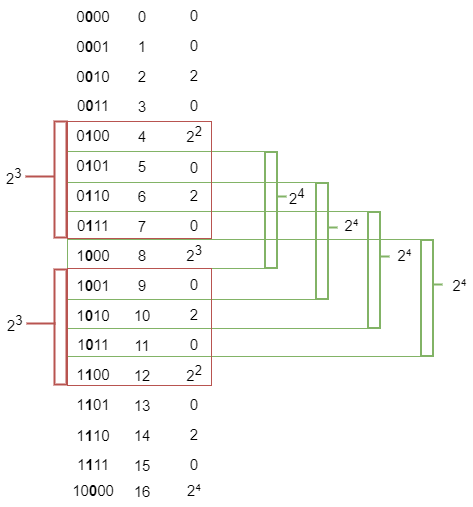
\includegraphics[width=0.6\textwidth]{Figures/Binomial_explanation.png} 
    \caption{This figure illustrates how the four factors in the denominator contains \(2^3\) and \(2^4\) or more 2 factors.} 
    \label{fig:n4j2} 
\end{figure}

Note that the four first numbers (\(\{0, 1, 2, 3\}\)) will be zero because non of the gates can be active, and thus the approach also holds for those cases.

With this we have shown that using the five qubit gate (see Figure \ref{fig:quad_cnot} to cover all possible combinations of four inputs, we can solve the \(j=3\) problem for any \(n \ge 4\). To complete the solution we also need to show the decomposition of the gate with four control qubits. For this we applied the general framework for decomposing any multi-qubit gates with n control bits presented in \cite[p.17-18]{barenco_elementary_1995}. The core of the method is the following identity:

\[
    \sum_{k_1}z_{k_1} - \sum_{k_1 < k_2}(z_{k_1} \oplus z_{k_2}) 
    + \sum_{k_1 < k_2 < k_3}(z_{k_1} \oplus z_{k_2}\oplus z_{k_3}) 
    - \; ... \;+ (-1)^{m-1} (z_{1} \oplus z_{2}\oplus \; ... \; \oplus z_{m})\] 

\[
= 2^{m-1}(x_1 \; \land \; x_1 \; \land \; ... \; \land \; x_m)    
\]
Where \(z_k\) is the \(k\)-th input qubit. For the case where \(m=4)\) we get the following equation:
\[
z_0 + z_1 + z_2 + z_4 - (z_0 \oplus z_1) - (z_0 \oplus z_2) - (z_0 \oplus z_3) - (z_1 \oplus z_2) - (z_1 \oplus z_3) - (z_2 \oplus z_3) 
\] 
\[
+ (z_0 \oplus z_1 \oplus z_2) + (z_0 \oplus z_1 \oplus z_3) + (z_1 \oplus z_2 \oplus z_3) - (z_0 \oplus z_1 \oplus z_2 \oplus z_3) 
\] 
\[ 
= 2^{3}(z_0 \; \land \; z_1 \; \land \; z_2 \; \land \; z_3)
\]
The circuit can with this be decomposed with CNOT gates and controlled rotation gates of the single qubit gate that the circuit is applying in the target qubit. For a unitary single qubit operation \(U\), the single qubit operator we need is the gate V such that \(U = V^{2m}\). In our case we need the \(X^{\frac{1}{2 \cdot 4}} = X^{\frac{1}{8}}\). Since CRX is not one of the elementary gates (CNOT or single qubit gate), we need to decompose the CRX gate. However, the decomposition of the CRX gate requires more gates than the CRZ decomposition \cite{liu_analysis_2024}. An idea is to change the standard basis of the target qubit to \(\{\ket{+}, \ket{-}\}\) with a Hadamard gate. After that, applying the CRZ gates has the same effect as CRX in the \(\{\ket{0}, \ket{1}\}\) basis. The basis is transformed back with another Hadamard gate to finish the algorithm. In that case \(V = Z^{\frac{1}{8}} = \begin{bmatrix}1 & 0 \\ 0 & e^{\frac{\pi}{8}i} \end{bmatrix}\).

The complete circuit can now be implemented by adding the V gate each time a positive term in the above identity is True and adding the \(V^{\dagger}\) when a negative term is True. The circuit is constructed by following the grey code sequence. The order can be reviewed in Table \ref{table:grey_code_truth}. A core idea is that CNOT is equvalent with the xor operator and it is unitary, menaing that applying the same CNOT a second time will recreate the previous state. The Finished circuit can be examined in Figure \ref{fig:quad_cnot_decomp}.

\begin{table}[htbp]
\caption{The order in which the cnot (xor) gates are applied can be derived from the grey code sequence as shown in this table}
\label{table:grey_code_truth}
\begin{center}
\begin{tabular}{|c|c|c|} 
 \hline
 Selected inputs & Boolean expression & Effect on target \\  
 \hline
 0000 & - & - \\ 
 \hline
 1000 & \(z_0\) & \(R_z(\frac{\pi}{8})\) \\
 \hline
 1100 & \(x_0 \oplus z_1\) & \(R_z(-\frac{\pi}{8})\) \\
 \hline
 0100 & \(z_1\) & \(R_z(\frac{\pi}{8})\) \\
 \hline
 0110 & \(z_1 \oplus z_2\) & \(R_z(-\frac{\pi}{8})\) \\
 \hline
 1110 & \(z_0 \oplus z_1 \oplus z_2\) & \(R_z(\frac{\pi}{8})\) \\
 \hline 
 1010 & \(z_0 \oplus z_2\) & \(R_z(-\frac{\pi}{8})\) \\
 \hline 
 0010 & \(z_2\) & \(R_z(\frac{\pi}{8})\) \\
 \hline
 0011 & \(z_2 \oplus z_3\) & \(R_z(-\frac{\pi}{8})\) \\
 \hline
 1011 & \(z_0 \oplus z_2 \oplus z_3\) & \(R_z(\frac{\pi}{8})\) \\
 \hline
 1111 & \(z_0 \oplus z_1 \oplus z_2 \otimes z_3\) & \(R_z(-\frac{\pi}{8})\) \\
 \hline
 0111 & \(z_1 \oplus z_2 \oplus z_3\) & \(R_z(\frac{\pi}{8})\) \\
 \hline
 0101 & \(z_1 \oplus z_3\) & \(R_z(-\frac{\pi}{8})\) \\
 \hline
 1101 & \(z_0 \oplus z_1 \oplus z_3\) & \(R_z(\frac{\pi}{8})\) \\
 \hline 
 1001 & \(z_0 \oplus z_3\) & \(R_z(-\frac{\pi}{8})\) \\
 \hline 
 0001 & \(z_3\) & \(R_z(\frac{\pi}{8})\) \\
 \hline
\end{tabular}
\end{center}
\end{table}

\begin{figure}[htbp] 
    \centering 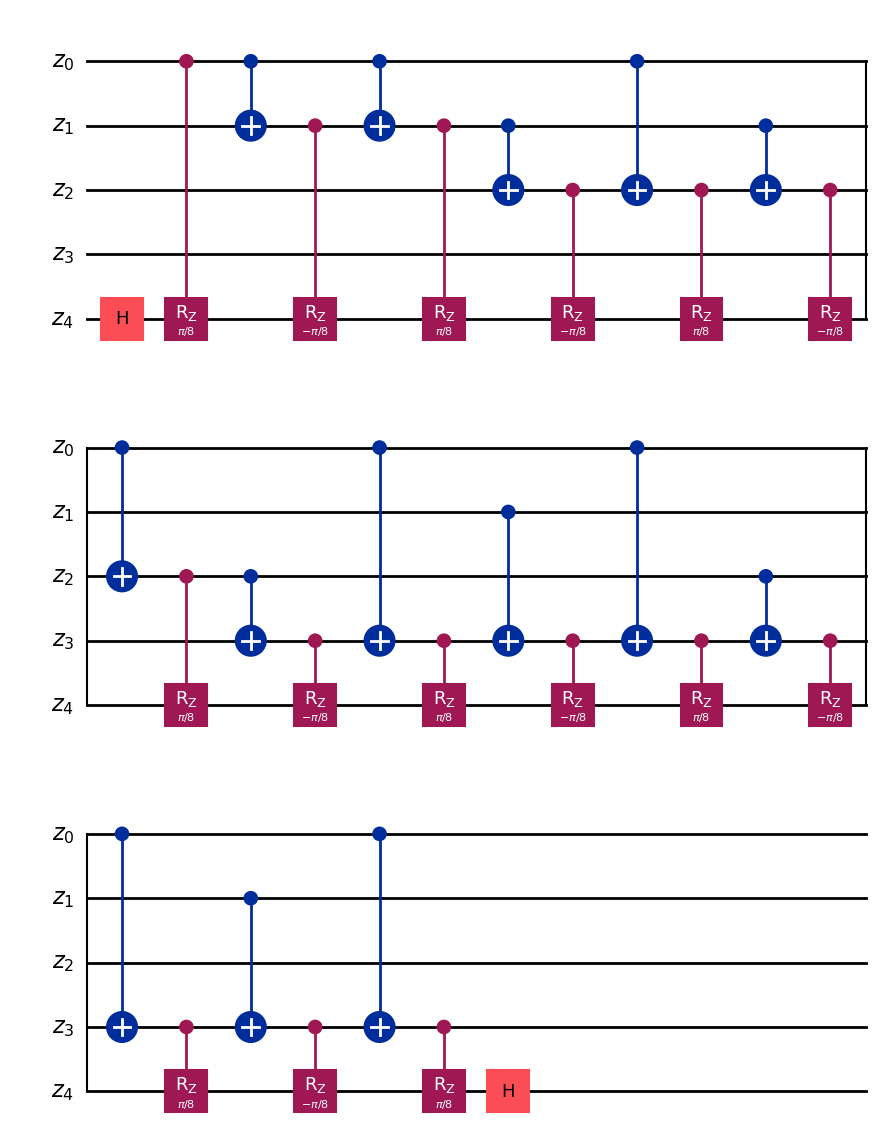
\includegraphics[width=1\textwidth]{Figures/quad_cnot_decomposition.png} 
    \caption{The decomposition of the quadruple CNOT gate.} 
    \label{fig:quad_cnot_decomp} 
\end{figure}
\newpage
\section{Conclusion}
During this project, we were able to find a brute force method for solving the popcount problem for \(j \in \{1, 2, 3\}\). The method covers all output combinations with controlled gates. The key that is utilized by this method is the connection between the binary bit positions and the binomial coefficient which counts the number of activated control gates. When we look at the odd/even pattern for \(\binom{\omega(z_n)}{8}\) follows a similar pattern with 8 consecutive odd numbers and even numbers. As a result we end up with the hypothesis that the brute force method generalizes to \(j \ge 1\) where the number of control qubits are given by \(2^{j-1}\). The general expression for the brute force method can, with this assumption, be expressed like this:

\[\ket{z_n, y_2} \xrightarrow{ET} 
    \begin{cases}
    \ket{z_n, 0} & 2^{j-1} > \omega(z_n) \ge 0 \\
    \ket{z_n} \otimes X^{\binom{\omega(z_n)}{2^{j-1}}}\ket{0} & \omega(z_n) \ge 2^{j-1}
    \end{cases}
\]

Future work would be to prove that the connection between the bit values of a binary and the binomial coefficient occurs for any bit position.

We were also able to show that the Quantum Fourier Transform can be used to solve the \(j=2\) problem instance with considerably less gates. This approach is however not feasible for any instances with \(j > 2\) because we would require at least one more qubit for every increase in \(j\).

\newpage


\bibliography{references}
\bibliographystyle{IEEEtran}

\newpage

\section{Appendix}

\subsubsection{Appendix A}
\label{appendix_a}

For running the simulation with Qiskit a jupyter notebook was created. In this appendix the exported version of the notebook can be reviewed.
The following libraries were imported:

    \begin{tcolorbox}[breakable, size=fbox, boxrule=1pt, pad at break*=1mm,colback=cellbackground, colframe=cellborder]
\prompt{In}{incolor}{19}{\boxspacing}
\begin{Verbatim}[commandchars=\\\{\}]
\PY{k+kn}{import} \PY{n+nn}{qiskit}
\PY{k+kn}{from} \PY{n+nn}{qiskit} \PY{k+kn}{import} \PY{n}{QuantumRegister}\PY{p}{,} \PY{n}{ClassicalRegister}\PY{p}{,} \PY{n}{QuantumCircuit}
\PY{k+kn}{import} \PY{n+nn}{numpy} \PY{k}{as} \PY{n+nn}{np}
\PY{k+kn}{import} \PY{n+nn}{matplotlib}\PY{n+nn}{.}\PY{n+nn}{pyplot} \PY{k}{as} \PY{n+nn}{plt}
\PY{k+kn}{from} \PY{n+nn}{qiskit\PYZus{}aer}\PY{n+nn}{.}\PY{n+nn}{primitives} \PY{k+kn}{import} \PY{n}{Sampler}
\PY{k+kn}{import} \PY{n+nn}{copy}
\PY{k+kn}{import} \PY{n+nn}{pandas} \PY{k}{as} \PY{n+nn}{pd}
\end{Verbatim}
\end{tcolorbox}

    The specific problem instance is defined:

    \begin{tcolorbox}[breakable, size=fbox, boxrule=1pt, pad at break*=1mm,colback=cellbackground, colframe=cellborder]
\prompt{In}{incolor}{20}{\boxspacing}
\begin{Verbatim}[commandchars=\\\{\}]
\PY{c+c1}{\PYZsh{} problem definition}
\PY{n}{n} \PY{o}{=} \PY{l+m+mi}{6}
\end{Verbatim}
\end{tcolorbox}

    Function to prepare the initial states of the circuit. It takes a numpy
array (input\_boolean) containing booleans representing the binary
string that should be prepared:

    \begin{tcolorbox}[breakable, size=fbox, boxrule=1pt, pad at break*=1mm,colback=cellbackground, colframe=cellborder]
\prompt{In}{incolor}{21}{\boxspacing}
\begin{Verbatim}[commandchars=\\\{\}]
\PY{k}{def} \PY{n+nf}{prepare\PYZus{}input\PYZus{}state}\PY{p}{(}\PY{n}{input\PYZus{}boolean}\PY{p}{:} \PY{n}{np}\PY{o}{.}\PY{n}{ndarray}\PY{p}{,} \PY{n}{qreg}\PY{p}{:} \PY{n}{QuantumRegister}\PY{p}{,} \PY{n}{qc}\PY{p}{:} \PY{n}{QuantumCircuit}\PY{p}{)}\PY{p}{:} 
    \PY{k}{for} \PY{n}{i}\PY{p}{,} \PY{n}{set\PYZus{}bit} \PY{o+ow}{in} \PY{n+nb}{enumerate}\PY{p}{(}\PY{n}{input\PYZus{}boolean}\PY{p}{)}\PY{p}{:}
        \PY{c+c1}{\PYZsh{} For each bit in the bit string}
        \PY{k}{if} \PY{n}{set\PYZus{}bit}\PY{p}{:}
            \PY{c+c1}{\PYZsh{} If the bit is set (True), then apply the bit flip to the corresponding qubit}
            \PY{n}{qc}\PY{o}{.}\PY{n}{x}\PY{p}{(}\PY{n}{qreg}\PY{p}{[}\PY{n}{i}\PY{p}{]}\PY{p}{)}
            
\end{Verbatim}
\end{tcolorbox}

    The following functions create the different circuits that solve the
popcount j=2 problem for \(n > 0, n \in \mathbb{Z}\).

    \begin{tcolorbox}[breakable, size=fbox, boxrule=1pt, pad at break*=1mm,colback=cellbackground, colframe=cellborder]
\prompt{In}{incolor}{22}{\boxspacing}
\begin{Verbatim}[commandchars=\\\{\}]
\PY{k}{def} \PY{n+nf}{create\PYZus{}QPE\PYZus{}popcount\PYZus{}circuit\PYZus{}rcx}\PY{p}{(}\PY{n}{qreg}\PY{p}{:} \PY{n}{QuantumRegister}\PY{p}{,} \PY{n}{qreg\PYZus{}result}\PY{p}{:} \PY{n}{QuantumRegister}\PY{p}{,} \PY{n}{creg}\PY{p}{:} \PY{n}{ClassicalRegister}\PY{p}{,} \PY{n}{qc}\PY{p}{:} \PY{n}{QuantumCircuit}\PY{p}{,} \PY{n}{n}\PY{p}{:} \PY{n+nb}{int}\PY{p}{)}\PY{p}{:}
    \PY{c+c1}{\PYZsh{} This function takes the quantum circuit as argument and applies the QFT solution using the CR\PYZus{}x(pi/2)}
    \PY{c+c1}{\PYZsh{} Note that the hadamard gates are not used in this case}
    \PY{k}{for} \PY{n}{control\PYZus{}q} \PY{o+ow}{in} \PY{n+nb}{range}\PY{p}{(}\PY{n}{n}\PY{p}{)}\PY{p}{:}
        \PY{c+c1}{\PYZsh{} Apply the crx gate with pi/2 as rotation angle (S gate) with each input qubit as control bit and the y\PYZus{}2 qubit as target.}
        \PY{n}{qc}\PY{o}{.}\PY{n}{crx}\PY{p}{(}\PY{n}{np}\PY{o}{.}\PY{n}{pi}\PY{o}{/}\PY{l+m+mi}{2}\PY{p}{,} \PY{n}{qreg}\PY{p}{[}\PY{n}{control\PYZus{}q}\PY{p}{]}\PY{p}{,} \PY{n}{qreg\PYZus{}result}\PY{p}{)}

    \PY{k}{for} \PY{n}{control\PYZus{}q} \PY{o+ow}{in} \PY{n+nb}{range}\PY{p}{(}\PY{n}{n}\PY{o}{\PYZhy{}}\PY{l+m+mi}{1}\PY{p}{)}\PY{p}{:}
        \PY{c+c1}{\PYZsh{} Add the CNOT operators for each input qubit as controll except one which serves as target to get the y\PYZus{}1 value.}
        \PY{n}{qc}\PY{o}{.}\PY{n}{cx}\PY{p}{(}\PY{n}{qreg}\PY{p}{[}\PY{n}{control\PYZus{}q}\PY{p}{]}\PY{p}{,} \PY{n}{qreg}\PY{p}{[}\PY{n}{n}\PY{o}{\PYZhy{}}\PY{l+m+mi}{1}\PY{p}{]}\PY{p}{)}

    \PY{c+c1}{\PYZsh{} Add the inverse controlled operation once qwith y\PYZus{}1 as controll and y\PYZus{}2 as target. }
    \PY{n}{qc}\PY{o}{.}\PY{n}{crx}\PY{p}{(}\PY{o}{\PYZhy{}}\PY{n}{np}\PY{o}{.}\PY{n}{pi}\PY{o}{/}\PY{l+m+mi}{2}\PY{p}{,} \PY{n}{qreg}\PY{p}{[}\PY{n}{n}\PY{o}{\PYZhy{}}\PY{l+m+mi}{1}\PY{p}{]}\PY{p}{,} \PY{n}{qreg\PYZus{}result}\PY{p}{)}
    \PY{c+c1}{\PYZsh{} The y\PYZus{}2 qubit is measured}
    \PY{n}{qc}\PY{o}{.}\PY{n}{measure}\PY{p}{(}\PY{n}{qreg\PYZus{}result}\PY{p}{,} \PY{n}{creg}\PY{p}{)}

\PY{k}{def} \PY{n+nf}{create\PYZus{}QPE\PYZus{}popcount\PYZus{}circuit\PYZus{}rcz}\PY{p}{(}\PY{n}{qreg}\PY{p}{:} \PY{n}{QuantumRegister}\PY{p}{,} \PY{n}{qreg\PYZus{}result}\PY{p}{:} \PY{n}{QuantumRegister}\PY{p}{,} \PY{n}{creg}\PY{p}{:} \PY{n}{ClassicalRegister}\PY{p}{,} \PY{n}{qc}\PY{p}{:} \PY{n}{QuantumCircuit}\PY{p}{,} \PY{n}{n}\PY{p}{:} \PY{n+nb}{int}\PY{p}{)}\PY{p}{:}
    \PY{c+c1}{\PYZsh{} This function takes the quantum circuit as argument and applies the QFT solution using the decomposition of CR\PYZus{}z(pi/2)}
    \PY{k}{for} \PY{n}{control\PYZus{}q} \PY{o+ow}{in} \PY{n+nb}{range}\PY{p}{(}\PY{n}{n}\PY{p}{)}\PY{p}{:}
        \PY{c+c1}{\PYZsh{} Apply the crz gate with pi/2 as rotation angle (S gate) with each input qubit as control bit and the y\PYZus{}2 qubit as target.}
        \PY{n}{qc}\PY{o}{.}\PY{n}{rz}\PY{p}{(}\PY{n}{np}\PY{o}{.}\PY{n}{pi}\PY{o}{/}\PY{l+m+mi}{4}\PY{p}{,} \PY{n}{qreg\PYZus{}result}\PY{p}{)}
        \PY{n}{qc}\PY{o}{.}\PY{n}{cx}\PY{p}{(}\PY{n}{qreg}\PY{p}{[}\PY{n}{control\PYZus{}q}\PY{p}{]}\PY{p}{,} \PY{n}{qreg\PYZus{}result}\PY{p}{)}
        \PY{n}{qc}\PY{o}{.}\PY{n}{rz}\PY{p}{(}\PY{o}{\PYZhy{}}\PY{n}{np}\PY{o}{.}\PY{n}{pi}\PY{o}{/}\PY{l+m+mi}{4}\PY{p}{,} \PY{n}{qreg\PYZus{}result}\PY{p}{)}
        \PY{n}{qc}\PY{o}{.}\PY{n}{cx}\PY{p}{(}\PY{n}{qreg}\PY{p}{[}\PY{n}{control\PYZus{}q}\PY{p}{]}\PY{p}{,} \PY{n}{qreg\PYZus{}result}\PY{p}{)}
        

    \PY{k}{for} \PY{n}{control\PYZus{}q} \PY{o+ow}{in} \PY{n+nb}{range}\PY{p}{(}\PY{n}{n}\PY{o}{\PYZhy{}}\PY{l+m+mi}{1}\PY{p}{)}\PY{p}{:}
        \PY{c+c1}{\PYZsh{} Add the CNOT operators for each input qubit as controll except one which serves as target to get the y\PYZus{}1 value.}
        \PY{n}{qc}\PY{o}{.}\PY{n}{cx}\PY{p}{(}\PY{n}{qreg}\PY{p}{[}\PY{n}{control\PYZus{}q}\PY{p}{]}\PY{p}{,} \PY{n}{qreg}\PY{p}{[}\PY{n}{n}\PY{o}{\PYZhy{}}\PY{l+m+mi}{1}\PY{p}{]}\PY{p}{)}

    \PY{c+c1}{\PYZsh{} Add the inverse controlled operation once qwith y\PYZus{}1 as controll and y\PYZus{}2 as target. }
    \PY{n}{qc}\PY{o}{.}\PY{n}{rz}\PY{p}{(}\PY{o}{\PYZhy{}}\PY{n}{np}\PY{o}{.}\PY{n}{pi}\PY{o}{/}\PY{l+m+mi}{4}\PY{p}{,} \PY{n}{qreg\PYZus{}result}\PY{p}{)}
    \PY{n}{qc}\PY{o}{.}\PY{n}{cx}\PY{p}{(}\PY{n}{qreg}\PY{p}{[}\PY{n}{n}\PY{o}{\PYZhy{}}\PY{l+m+mi}{1}\PY{p}{]}\PY{p}{,} \PY{n}{qreg\PYZus{}result}\PY{p}{)}
    \PY{n}{qc}\PY{o}{.}\PY{n}{rz}\PY{p}{(}\PY{n}{np}\PY{o}{.}\PY{n}{pi}\PY{o}{/}\PY{l+m+mi}{4}\PY{p}{,} \PY{n}{qreg\PYZus{}result}\PY{p}{)}
    \PY{n}{qc}\PY{o}{.}\PY{n}{cx}\PY{p}{(}\PY{n}{qreg}\PY{p}{[}\PY{n}{n}\PY{o}{\PYZhy{}}\PY{l+m+mi}{1}\PY{p}{]}\PY{p}{,} \PY{n}{qreg\PYZus{}result}\PY{p}{)}
    \PY{c+c1}{\PYZsh{} The y\PYZus{}2 qubit is measured}
    \PY{n}{qc}\PY{o}{.}\PY{n}{measure}\PY{p}{(}\PY{n}{qreg\PYZus{}result}\PY{p}{,} \PY{n}{creg}\PY{p}{)}
\end{Verbatim}
\end{tcolorbox}

    Instantiate the registers and circuit objects and prepare the circuit.
Note that the qubits are divided into two registers: One for the n
inputs and one for the single qubit output

    \begin{tcolorbox}[breakable, size=fbox, boxrule=1pt, pad at break*=1mm,colback=cellbackground, colframe=cellborder]
\prompt{In}{incolor}{29}{\boxspacing}
\begin{Verbatim}[commandchars=\\\{\}]
\PY{n}{qreg} \PY{o}{=} \PY{n}{QuantumRegister}\PY{p}{(}\PY{n}{n}\PY{p}{,} \PY{n}{name}\PY{o}{=}\PY{l+s+s2}{\PYZdq{}}\PY{l+s+s2}{z}\PY{l+s+s2}{\PYZdq{}}\PY{p}{)}
\PY{n}{qreg\PYZus{}result} \PY{o}{=} \PY{n}{QuantumRegister}\PY{p}{(}\PY{l+m+mi}{1}\PY{p}{,} \PY{n}{name}\PY{o}{=}\PY{l+s+s2}{\PYZdq{}}\PY{l+s+s2}{y\PYZus{}2}\PY{l+s+s2}{\PYZdq{}}\PY{p}{)}
\PY{n}{creg} \PY{o}{=} \PY{n}{ClassicalRegister}\PY{p}{(}\PY{l+m+mi}{1}\PY{p}{,} \PY{n}{name}\PY{o}{=}\PY{l+s+s2}{\PYZdq{}}\PY{l+s+s2}{Result}\PY{l+s+s2}{\PYZdq{}}\PY{p}{)}
\PY{n}{qc} \PY{o}{=} \PY{n}{QuantumCircuit}\PY{p}{(}\PY{n}{qreg}\PY{p}{,} \PY{n}{qreg\PYZus{}result}\PY{p}{,} \PY{n}{creg}\PY{p}{,} \PY{n}{name}\PY{o}{=}\PY{l+s+s2}{\PYZdq{}}\PY{l+s+s2}{QFT popcount solution with crz decomposition}\PY{l+s+s2}{\PYZdq{}}\PY{p}{)}

\PY{n}{create\PYZus{}QPE\PYZus{}popcount\PYZus{}circuit\PYZus{}rcz}\PY{p}{(}\PY{n}{qreg}\PY{p}{,} \PY{n}{qreg\PYZus{}result}\PY{p}{,} \PY{n}{creg}\PY{p}{,} \PY{n}{qc}\PY{p}{,} \PY{n}{n}\PY{p}{)}
\PY{n}{qc}\PY{o}{.}\PY{n}{draw}\PY{p}{(}\PY{l+s+s2}{\PYZdq{}}\PY{l+s+s2}{mpl}\PY{l+s+s2}{\PYZdq{}}\PY{p}{)}
\end{Verbatim}
\end{tcolorbox}
    See figure \ref{fig:qft_crz_circuit_drawing} for the output image from this cell.

    Next, all different \(2^n\) input combinations are generated an stored
as numpy array

    \begin{tcolorbox}[breakable, size=fbox, boxrule=1pt, pad at break*=1mm,colback=cellbackground, colframe=cellborder]
\prompt{In}{incolor}{ }{\boxspacing}
\begin{Verbatim}[commandchars=\\\{\}]
\PY{c+c1}{\PYZsh{} The following lines generates all 2**n input combinations}
\PY{n}{input\PYZus{}states} \PY{o}{=} \PY{n}{np}\PY{o}{.}\PY{n}{empty}\PY{p}{(}\PY{p}{(}\PY{l+m+mi}{2}\PY{o}{*}\PY{o}{*}\PY{n}{n}\PY{p}{,} \PY{n}{n}\PY{p}{)}\PY{p}{,} \PY{n}{dtype}\PY{o}{=}\PY{n+nb}{bool}\PY{p}{)}
\PY{k}{for} \PY{n}{i} \PY{o+ow}{in} \PY{n+nb}{range}\PY{p}{(}\PY{l+m+mi}{2}\PY{o}{*}\PY{o}{*}\PY{n}{n}\PY{p}{)}\PY{p}{:}
    \PY{n}{input\PYZus{}states}\PY{p}{[}\PY{n}{i}\PY{p}{,} \PY{p}{:}\PY{p}{]} \PY{o}{=} \PY{n}{np}\PY{o}{.}\PY{n}{array}\PY{p}{(}\PY{n+nb}{list}\PY{p}{(}\PY{n+nb}{bin}\PY{p}{(}\PY{n}{i}\PY{p}{)}\PY{p}{[}\PY{l+m+mi}{2}\PY{p}{:}\PY{p}{]}\PY{o}{.}\PY{n}{zfill}\PY{p}{(}\PY{n}{n}\PY{p}{)}\PY{p}{)}\PY{p}{,} \PY{n}{dtype}\PY{o}{=}\PY{n+nb}{int}\PY{p}{)}\PY{o}{.}\PY{n}{astype}\PY{p}{(}\PY{n+nb}{bool}\PY{p}{)}
\end{Verbatim}
\end{tcolorbox}

This cell verifies that there are no redundant inputs in the list

    \begin{tcolorbox}[breakable, size=fbox, boxrule=1pt, pad at break*=1mm,colback=cellbackground, colframe=cellborder]
\prompt{In}{incolor}{7}{\boxspacing}
\begin{Verbatim}[commandchars=\\\{\}]
\PY{n}{test\PYZus{}list} \PY{o}{=} \PY{p}{[}\PY{p}{]}
\PY{k}{for} \PY{n}{input\PYZus{}state} \PY{o+ow}{in} \PY{n}{input\PYZus{}states}\PY{p}{:}
    \PY{n}{test\PYZus{}list}\PY{o}{.}\PY{n}{append}\PY{p}{(}\PY{n+nb}{int}\PY{p}{(}\PY{l+s+s2}{\PYZdq{}}\PY{l+s+s2}{\PYZdq{}}\PY{o}{.}\PY{n}{join}\PY{p}{(}\PY{n}{input\PYZus{}state}\PY{o}{.}\PY{n}{astype}\PY{p}{(}\PY{n+nb}{int}\PY{p}{)}\PY{o}{.}\PY{n}{astype}\PY{p}{(}\PY{n+nb}{str}\PY{p}{)}\PY{p}{)}\PY{p}{,} \PY{l+m+mi}{2}\PY{p}{)}\PY{p}{)}

\PY{n}{cur\PYZus{}length} \PY{o}{=} \PY{n+nb}{len}\PY{p}{(}\PY{n}{test\PYZus{}list}\PY{p}{)}
\PY{n}{actual\PYZus{}unique\PYZus{}lenght} \PY{o}{=} \PY{n+nb}{len}\PY{p}{(}\PY{n+nb}{set}\PY{p}{(}\PY{n}{test\PYZus{}list}\PY{p}{)}\PY{p}{)}
\PY{k}{if} \PY{o+ow}{not} \PY{p}{(}\PY{n}{cur\PYZus{}length} \PY{o}{==} \PY{n}{actual\PYZus{}unique\PYZus{}lenght}\PY{p}{)}\PY{p}{:}
    \PY{n+nb}{print}\PY{p}{(}\PY{l+s+s2}{\PYZdq{}}\PY{l+s+s2}{There is a mistake in the generator function}\PY{l+s+s2}{\PYZdq{}}\PY{p}{)}
\end{Verbatim}
\end{tcolorbox}

Finally the circuit is tested by running the simulation for every possible input combination. The results are stored in a pandas dataframe and saved to a csv file in the current working directory with filename "popcount\_QPE\_analysis\_n\{n\}.csv" (\{n\} depends on n)

    \begin{tcolorbox}[breakable, size=fbox, boxrule=1pt, pad at break*=1mm,colback=cellbackground, colframe=cellborder]
\prompt{In}{incolor}{10}{\boxspacing}
\begin{Verbatim}[commandchars=\\\{\}]
\PY{n}{results} \PY{o}{=} \PY{p}{\PYZob{}}\PY{l+s+s2}{\PYZdq{}}\PY{l+s+s2}{Input\PYZus{}dec}\PY{l+s+s2}{\PYZdq{}} \PY{p}{:} \PY{p}{[}\PY{p}{]}\PY{p}{,} \PY{l+s+s2}{\PYZdq{}}\PY{l+s+s2}{Input\PYZus{}bin}\PY{l+s+s2}{\PYZdq{}} \PY{p}{:} \PY{p}{[}\PY{p}{]}\PY{p}{,} \PY{l+s+s2}{\PYZdq{}}\PY{l+s+s2}{Hamming\PYZus{}weight}\PY{l+s+s2}{\PYZdq{}} \PY{p}{:} \PY{p}{[}\PY{p}{]}\PY{p}{,} \PY{l+s+s2}{\PYZdq{}}\PY{l+s+s2}{Expected\PYZus{}output}\PY{l+s+s2}{\PYZdq{}} \PY{p}{:} \PY{p}{[}\PY{p}{]}\PY{p}{,} \PY{l+s+s2}{\PYZdq{}}\PY{l+s+s2}{Measured\PYZus{}result}\PY{l+s+s2}{\PYZdq{}} \PY{p}{:} \PY{p}{[}\PY{p}{]}\PY{p}{\PYZcb{}}
\PY{k}{for} \PY{n}{input\PYZus{}state} \PY{o+ow}{in} \PY{n}{input\PYZus{}states}\PY{p}{:}
    \PY{n}{cur\PYZus{}input\PYZus{}decimal} \PY{o}{=} \PY{n+nb}{int}\PY{p}{(}\PY{l+s+s2}{\PYZdq{}}\PY{l+s+s2}{\PYZdq{}}\PY{o}{.}\PY{n}{join}\PY{p}{(}\PY{n}{input\PYZus{}state}\PY{o}{.}\PY{n}{astype}\PY{p}{(}\PY{n+nb}{int}\PY{p}{)}\PY{o}{.}\PY{n}{astype}\PY{p}{(}\PY{n+nb}{str}\PY{p}{)}\PY{p}{)}\PY{p}{,} \PY{l+m+mi}{2}\PY{p}{)}
    \PY{n}{cur\PYZus{}hamming\PYZus{}weight} \PY{o}{=} \PY{n}{np}\PY{o}{.}\PY{n}{sum}\PY{p}{(}\PY{n}{input\PYZus{}state}\PY{o}{.}\PY{n}{astype}\PY{p}{(}\PY{n+nb}{int}\PY{p}{)}\PY{p}{)}
    \PY{c+c1}{\PYZsh{} Here the output bit is determined by checking if the hamming weight value has the second bit set to 1}
    \PY{n}{expected\PYZus{}output} \PY{o}{=} \PY{n+nb}{int}\PY{p}{(}\PY{n+nb}{bin}\PY{p}{(}\PY{n}{np}\PY{o}{.}\PY{n}{sum}\PY{p}{(}\PY{n}{input\PYZus{}state}\PY{o}{.}\PY{n}{astype}\PY{p}{(}\PY{n+nb}{int}\PY{p}{)}\PY{p}{)}\PY{p}{)}\PY{p}{[}\PY{l+m+mi}{2}\PY{p}{:}\PY{p}{]}\PY{o}{.}\PY{n}{zfill}\PY{p}{(}\PY{n}{n}\PY{p}{)}\PY{p}{[}\PY{o}{\PYZhy{}}\PY{l+m+mi}{2}\PY{p}{]}\PY{p}{)}

    \PY{n}{cur\PYZus{}qreg} \PY{o}{=} \PY{n}{QuantumRegister}\PY{p}{(}\PY{n}{n}\PY{o}{+}\PY{l+m+mi}{1}\PY{p}{,} \PY{n}{name}\PY{o}{=}\PY{l+s+s2}{\PYZdq{}}\PY{l+s+s2}{qreg}\PY{l+s+s2}{\PYZdq{}}\PY{p}{)}
    \PY{n}{cur\PYZus{}creg} \PY{o}{=} \PY{n}{ClassicalRegister}\PY{p}{(}\PY{l+m+mi}{1}\PY{p}{,} \PY{n}{name}\PY{o}{=}\PY{l+s+s2}{\PYZdq{}}\PY{l+s+s2}{creg}\PY{l+s+s2}{\PYZdq{}}\PY{p}{)}
    \PY{n}{cur\PYZus{}qc} \PY{o}{=} \PY{n}{QuantumCircuit}\PY{p}{(}\PY{n}{qreg}\PY{p}{,} \PY{n}{creg}\PY{p}{)}

    \PY{n}{prepare\PYZus{}input\PYZus{}state}\PY{p}{(}\PY{n}{input\PYZus{}state}\PY{p}{,} \PY{n}{cur\PYZus{}qreg}\PY{p}{,} \PY{n}{cur\PYZus{}qc}\PY{p}{)}

    \PY{n}{create\PYZus{}QPE\PYZus{}popcount\PYZus{}circuit}\PY{p}{(}\PY{n}{cur\PYZus{}qreg}\PY{p}{,} \PY{n}{cur\PYZus{}creg}\PY{p}{,} \PY{n}{cur\PYZus{}qc}\PY{p}{,} \PY{n}{n}\PY{p}{)}
    \PY{n}{result} \PY{o}{=} \PY{n}{Sampler}\PY{p}{(}\PY{p}{)}\PY{o}{.}\PY{n}{run}\PY{p}{(}\PY{p}{[}\PY{n}{cur\PYZus{}qc}\PY{p}{]}\PY{p}{,} \PY{n}{shots}\PY{o}{=}\PY{l+m+mi}{500}\PY{p}{)}\PY{o}{.}\PY{n}{result}\PY{p}{(}\PY{p}{)}

    \PY{n}{results}\PY{p}{[}\PY{l+s+s2}{\PYZdq{}}\PY{l+s+s2}{Input\PYZus{}dec}\PY{l+s+s2}{\PYZdq{}}\PY{p}{]}\PY{o}{.}\PY{n}{append}\PY{p}{(}\PY{n}{cur\PYZus{}input\PYZus{}decimal}\PY{p}{)}
    \PY{n}{results}\PY{p}{[}\PY{l+s+s2}{\PYZdq{}}\PY{l+s+s2}{Input\PYZus{}bin}\PY{l+s+s2}{\PYZdq{}}\PY{p}{]}\PY{o}{.}\PY{n}{append}\PY{p}{(}\PY{l+s+s2}{\PYZdq{}}\PY{l+s+s2}{\PYZdq{}}\PY{o}{.}\PY{n}{join}\PY{p}{(}\PY{n}{input\PYZus{}state}\PY{o}{.}\PY{n}{astype}\PY{p}{(}\PY{n+nb}{int}\PY{p}{)}\PY{o}{.}\PY{n}{astype}\PY{p}{(}\PY{n+nb}{str}\PY{p}{)}\PY{p}{)}\PY{p}{)}
    \PY{n}{results}\PY{p}{[}\PY{l+s+s2}{\PYZdq{}}\PY{l+s+s2}{Hamming\PYZus{}weight}\PY{l+s+s2}{\PYZdq{}}\PY{p}{]}\PY{o}{.}\PY{n}{append}\PY{p}{(}\PY{n}{cur\PYZus{}hamming\PYZus{}weight}\PY{p}{)}
    \PY{n}{results}\PY{p}{[}\PY{l+s+s2}{\PYZdq{}}\PY{l+s+s2}{Expected\PYZus{}output}\PY{l+s+s2}{\PYZdq{}}\PY{p}{]}\PY{o}{.}\PY{n}{append}\PY{p}{(}\PY{n}{expected\PYZus{}output}\PY{p}{)}
    \PY{n}{measured\PYZus{}keys} \PY{o}{=} \PY{n}{result}\PY{o}{.}\PY{n}{quasi\PYZus{}dists}\PY{p}{[}\PY{l+m+mi}{0}\PY{p}{]}\PY{o}{.}\PY{n}{keys}\PY{p}{(}\PY{p}{)}
    \PY{k}{if} \PY{n+nb}{len}\PY{p}{(}\PY{n}{measured\PYZus{}keys}\PY{p}{)} \PY{o}{\PYZgt{}} \PY{l+m+mi}{1}\PY{p}{:}
        \PY{n}{results}\PY{p}{[}\PY{l+s+s2}{\PYZdq{}}\PY{l+s+s2}{Measured\PYZus{}result}\PY{l+s+s2}{\PYZdq{}}\PY{p}{]}\PY{o}{.}\PY{n}{append}\PY{p}{(}\PY{l+m+mi}{1}\PY{o}{/}\PY{l+m+mi}{2}\PY{p}{)}
    \PY{k}{else}\PY{p}{:}
        \PY{n}{results}\PY{p}{[}\PY{l+s+s2}{\PYZdq{}}\PY{l+s+s2}{Measured\PYZus{}result}\PY{l+s+s2}{\PYZdq{}}\PY{p}{]}\PY{o}{.}\PY{n}{append}\PY{p}{(}\PY{n+nb}{list}\PY{p}{(}\PY{n}{measured\PYZus{}keys}\PY{p}{)}\PY{p}{[}\PY{l+m+mi}{0}\PY{p}{]}\PY{p}{)}

\PY{n}{results\PYZus{}df} \PY{o}{=} \PY{n}{pd}\PY{o}{.}\PY{n}{DataFrame}\PY{p}{(}\PY{n}{results}\PY{p}{)}
\PY{n}{results\PYZus{}df}\PY{o}{.}\PY{n}{to\PYZus{}csv}\PY{p}{(}\PY{l+s+sa}{f}\PY{l+s+s2}{\PYZdq{}}\PY{l+s+s2}{popcount\PYZus{}QPE\PYZus{}analysis\PYZus{}n}\PY{l+s+si}{\PYZob{}}\PY{n}{n}\PY{l+s+si}{\PYZcb{}}\PY{l+s+s2}{.csv}\PY{l+s+s2}{\PYZdq{}}\PY{p}{)}
\PY{n}{results\PYZus{}df}
\end{Verbatim}
\end{tcolorbox}

            \begin{tcolorbox}[breakable, size=fbox, boxrule=.5pt, pad at break*=1mm, opacityfill=0]
\prompt{Out}{outcolor}{10}{\boxspacing}
\begin{Verbatim}[commandchars=\\\{\}]
    Input\_dec Input\_bin  Hamming\_weight  Expected\_output  Measured\_result
0           0    000000               0                0                0
1           1    000001               1                0                0
2           2    000010               1                0                0
3           3    000011               2                1                1
4           4    000100               1                0                0
..        {\ldots}       {\ldots}             {\ldots}              {\ldots}              {\ldots}
59         59    111011               5                0                0
60         60    111100               4                0                0
61         61    111101               5                0                0
62         62    111110               5                0                0
63         63    111111               6                1                1

[64 rows x 5 columns]
\end{Verbatim}
\end{tcolorbox}
        
    \begin{tcolorbox}[breakable, size=fbox, boxrule=1pt, pad at break*=1mm,colback=cellbackground, colframe=cellborder]
\prompt{In}{incolor}{12}{\boxspacing}
\begin{Verbatim}[commandchars=\\\{\}]
\PY{n}{results\PYZus{}df}\PY{o}{.}\PY{n}{groupby}\PY{p}{(}\PY{p}{[}\PY{l+s+s2}{\PYZdq{}}\PY{l+s+s2}{Hamming\PYZus{}weight}\PY{l+s+s2}{\PYZdq{}}\PY{p}{]}\PY{p}{)}\PY{p}{[}\PY{p}{[}\PY{l+s+s2}{\PYZdq{}}\PY{l+s+s2}{Expected\PYZus{}output}\PY{l+s+s2}{\PYZdq{}}\PY{p}{,} \PY{l+s+s2}{\PYZdq{}}\PY{l+s+s2}{Measured\PYZus{}result}\PY{l+s+s2}{\PYZdq{}}\PY{p}{]}\PY{p}{]}\PY{o}{.}\PY{n}{mean}\PY{p}{(}\PY{p}{)}
\end{Verbatim}
\end{tcolorbox}

            \begin{tcolorbox}[breakable, size=fbox, boxrule=.5pt, pad at break*=1mm, opacityfill=0]
\prompt{Out}{outcolor}{12}{\boxspacing}
\begin{Verbatim}[commandchars=\\\{\}]
                Expected\_output  Measured\_result
Hamming\_weight
0                           0.0              0.0
1                           0.0              0.0
2                           1.0              1.0
3                           1.0              1.0
4                           0.0              0.0
5                           0.0              0.0
6                           1.0              1.0
\end{Verbatim}
\end{tcolorbox} 

\begin{tcolorbox}[breakable, size=fbox, boxrule=1pt, pad at break*=1mm,colback=cellbackground, colframe=cellborder]
\prompt{In}{incolor}{12}{\boxspacing}
\begin{Verbatim}[commandchars=\\\{\}]
\PY{n}{results\PYZus{}df}\PY{o}{.}\PY{n}{groupby}\PY{p}{(}\PY{p}{[}\PY{l+s+s2}{\PYZdq{}}\PY{l+s+s2}{Hamming\PYZus{}weight}\PY{l+s+s2}{\PYZdq{}}\PY{p}{]}\PY{p}{)}\PY{p}{[}\PY{p}{[}\PY{l+s+s2}{\PYZdq{}}\PY{l+s+s2}{Expected\PYZus{}output}\PY{l+s+s2}{\PYZdq{}}\PY{p}{,} \PY{l+s+s2}{\PYZdq{}}\PY{l+s+s2}{Measured\PYZus{}result}\PY{l+s+s2}{\PYZdq{}}\PY{p}{]}\PY{p}{]}\PY{o}{.}\PY{n}{mean}\PY{p}{(}\PY{p}{)}
\end{Verbatim}
\end{tcolorbox}

\subsubsection{Appendix B}
\label{compact_margolis_solution_code}
Code for the compact margolis solution\ref{fig:simplified_margolis}:
\begin{tcolorbox}[breakable, size=fbox, boxrule=1pt, pad at break*=1mm,colback=cellbackground, colframe=cellborder]
\prompt{In}{incolor}{13}{\boxspacing}
\begin{Verbatim}[commandchars=\\\{\}]
def create_QPE_popcount_circuit(qreg: QuantumRegister, creg: ClassicalRegister, qc: QuantumCircuit, n: int):
    qc.ry(np.pi/4,qreg[3])
    qc.cx(qreg[1],qreg[3])
    qc.cx(qreg[2],qreg[3])
    qc.ry(np.pi/4,qreg[3])
    qc.cx(qreg[0],qreg[3])
    qc.ry(-np.pi/4,qreg[3])
    qc.cx(qreg[1],qreg[3])
    qc.ry(np.pi/4,qreg[3])
    qc.cx(qreg[1],qreg[3])
    qc.ry(-np.pi/4,qreg[3])
    qc.cx(qreg[2],qreg[3]) 
    qc.ry(-np.pi/4,qreg[3])
    qc.measure(qreg[n], creg)
\end{Verbatim}
\end{tcolorbox}
Results for the compact margolis solution:
            \begin{tcolorbox}[breakable, size=fbox, boxrule=.5pt, pad at break*=1mm, opacityfill=0]
\prompt{Out}{outcolor}{13}{\boxspacing}
\begin{Verbatim}[commandchars=\\\{\}]
	Expected_output	Measured_result
Hamming_weight		
0	0.0	0.0
1	0.0	0.0
2	1.0	1.0
3	1.0	1.0
\end{Verbatim}
\end{tcolorbox} 
\end{document}
